% Options for packages loaded elsewhere
\PassOptionsToPackage{unicode}{hyperref}
\PassOptionsToPackage{hyphens}{url}
%
\documentclass[
]{article}
\usepackage{lmodern}
\usepackage{amssymb,amsmath}
\usepackage{ifxetex,ifluatex}
\ifnum 0\ifxetex 1\fi\ifluatex 1\fi=0 % if pdftex
  \usepackage[T1]{fontenc}
  \usepackage[utf8]{inputenc}
  \usepackage{textcomp} % provide euro and other symbols
\else % if luatex or xetex
  \usepackage{unicode-math}
  \defaultfontfeatures{Scale=MatchLowercase}
  \defaultfontfeatures[\rmfamily]{Ligatures=TeX,Scale=1}
\fi
% Use upquote if available, for straight quotes in verbatim environments
\IfFileExists{upquote.sty}{\usepackage{upquote}}{}
\IfFileExists{microtype.sty}{% use microtype if available
  \usepackage[]{microtype}
  \UseMicrotypeSet[protrusion]{basicmath} % disable protrusion for tt fonts
}{}
\makeatletter
\@ifundefined{KOMAClassName}{% if non-KOMA class
  \IfFileExists{parskip.sty}{%
    \usepackage{parskip}
  }{% else
    \setlength{\parindent}{0pt}
    \setlength{\parskip}{6pt plus 2pt minus 1pt}}
}{% if KOMA class
  \KOMAoptions{parskip=half}}
\makeatother
\usepackage{xcolor}
\IfFileExists{xurl.sty}{\usepackage{xurl}}{} % add URL line breaks if available
\IfFileExists{bookmark.sty}{\usepackage{bookmark}}{\usepackage{hyperref}}
\hypersetup{
  pdftitle={A Comparison of GMAC and ADDIS},
  pdfauthor={Jarred Kvamme, University of Idaho},
  hidelinks,
  pdfcreator={LaTeX via pandoc}}
\urlstyle{same} % disable monospaced font for URLs
\usepackage[margin=1in]{geometry}
\usepackage{longtable,booktabs}
% Correct order of tables after \paragraph or \subparagraph
\usepackage{etoolbox}
\makeatletter
\patchcmd\longtable{\par}{\if@noskipsec\mbox{}\fi\par}{}{}
\makeatother
% Allow footnotes in longtable head/foot
\IfFileExists{footnotehyper.sty}{\usepackage{footnotehyper}}{\usepackage{footnote}}
\makesavenoteenv{longtable}
\usepackage{graphicx,grffile}
\makeatletter
\def\maxwidth{\ifdim\Gin@nat@width>\linewidth\linewidth\else\Gin@nat@width\fi}
\def\maxheight{\ifdim\Gin@nat@height>\textheight\textheight\else\Gin@nat@height\fi}
\makeatother
% Scale images if necessary, so that they will not overflow the page
% margins by default, and it is still possible to overwrite the defaults
% using explicit options in \includegraphics[width, height, ...]{}
\setkeys{Gin}{width=\maxwidth,height=\maxheight,keepaspectratio}
% Set default figure placement to htbp
\makeatletter
\def\fps@figure{htbp}
\makeatother
\setlength{\emergencystretch}{3em} % prevent overfull lines
\providecommand{\tightlist}{%
  \setlength{\itemsep}{0pt}\setlength{\parskip}{0pt}}
\setcounter{secnumdepth}{-\maxdimen} % remove section numbering

\title{A Comparison of GMAC and ADDIS}
\author{Jarred Kvamme, University of Idaho}
\date{9/22/2021}

\begin{document}
\maketitle

\section*{1. Overview}

Both MRPC-LOND and MRPC-ADDIS techniques inferred a large number of
trans mediated trios. The trans-mediation model has been previously
identified, but is not the commonly ackowledged mode of mediation. Since
this result is surprising relative to the existing literature, we sought
to apply another method for inferring mediation on a subset of GTEx
trios analyzed herein by MRPC. The Genomic Mediation analysis with
Adaptive Confounding (GMAC) algorithm allows for a unique selection of a
subset of potential confounders, \({\bf X_{ij}}\) from a larger
covariate pool, \({\bf H}\), for each trio. By taking advantage of the
Principle of Mendelian Randomization, the authors filter \({\bf H}\) by
removing common child and intermediate confounding variables (e.g
variables associated with the eQTL as well as the cis/trans genes).
Post-filtering, GMAC preforms a mediation test on the edge between the
cis gene and trans gene via the regression of the trans-gene \(T_j\) on
the cis-eQTL \(L_i\), cis-gene \(C_i\), and the set of adaptively
selected confounders \({\bf X_{ij}}\):

\begin{eqnarray} T_j = \beta_0 + \beta_1 C_i + \beta_2 L_i + {\bf \Gamma} {\bf X}_{ij} + \epsilon \end{eqnarray}

The mediation statistic is the observed \(t\)-value of the cis-gene
coefficient \(\beta_1\). A null distribution for no-mediation is
constructed by iteratively permuting the values of the cis-transcript
within each genotype and repeating the above regression. The authors
argue that the permutation of the cis-transcript within the genotypes of
the cis-eQTL removes the association between the cis and trans gene
transcripts while preserving the higher order associations with the
cis-eQTL. The resulting permutation test for mediation compares the
observed relationship between the trans and cis gene to a null
distribution constructed from a model with no association and assuming
that possible confounding has been well adjusted via the selected
covariates.

It is important to note that the above mediation test describes only the
association between cis-gene and trans-gene transcripts
(\(C_i \leftrightarrow T_j\) ) and does not consider possible effects
between the cis-eQTL and the cis-gene transcript
(\(L_i \rightarrow C_i\)), or the cis-eQTL and trans-gene transcript
(\(L_i \rightarrow T_j\)).

\section*{2. Methods}
\subsection*{2.1 Applying GMAC to GTEx Trios}

To compare the GMAC and MRPC algorithms, we applied the GMAC algorithm
to the top five GTEx tissues by sample size. Following with the creators
of GMAC, we used the full set of principle components retained from the
PCA of the expression matrix as the covariate pool, and three additional
known confounders: the PCR used, the platform used, and sex of the
individual in each sample (Yang et al. 2017).

Consistent with Yang et al. (2017), the analysis was preformed using a
common child and intermediate variable filtering FDR of \(10\%\) and a
confounder selection FDR of \(5\%\) for each trio. Each trio supplied to
GMAC consisted of the cis-QTL and the PEER normalized cis and trans gene
transcripts with the highest association to the eQTL. To mitigate
missing values in the eQTL matrix, multiple imputation of the matrix of
unique cis-eQTLs was preformed via multiple correspondence analysis
(MCA) prior to its use in GMAC (Josse, Husson, and others 2016). The
analysis was preformed twice on each trio, first with the cis gene as
the mediator and second with the trans gene as the mediator. This
allowed for GMAC inferred trios to be decomposed into the three
groupings used under MRPC: 1) Cis-gene mediation, 2) Trans-gene
mediation, 3) both (undirected).

\subsection*{2.2 Comparison of GMAC and MRPC Results}

After applying GMAC to each tissue, the false discovery rate among the
retained mediation p-values was controlled at the more liberal rate of
\(10\%\) (Yang et al. 2017). Each trio determined to have significant
mediation after FDR filtering was compared with the regulatory network
type inferred by MRPC-ADDIS. MRPC-ADDIS can infer three types of
regulatory networks that contain an edge between the cis and trans gene
(M1, M2, or M4). Since GMAC considers only the presence of the edge and
not its direction, trios inferred to be one of M1, M2, or M4 under
ADDIS, that were also significant under GMAC, were considered consistent
(e.g \(C_i \rightarrow T_j\); \(T_j \rightarrow C_i\);
\(C_i \leftrightarrow T_j\) are synonymous under GMAC).

\subsection*{2.3 Simulations}

\indent \(\bullet\) The Small True Model Simulation (STM)

To further understand the conflict in edge determination between
MRPC-ADDIS and GMAC, we simulated the mediation test - the test for the
\(\beta_1\) coefficient in the presence of all adaptively selected
confounders, \({\bf X}_{ij}\), as described by the regression in
\textbf{eq (1)} - under two different scenarios. (i) To observe the
predictive power of the mediation test when the trans gene comes from a
set of explanatory variables smaller than those in \({\bf X}_{ij}\), We
simulated the trans gene of each trio using the linear relationship:

\begin{eqnarray} T^{\ast}_{j} = \hat{\beta_0}+\hat{\beta_1}C_i + \hat{\beta_2}L_i + \hat{{\bf\Gamma}}_W {\bf W}_{ij} +\epsilon  \end{eqnarray}

where \(T^{\ast}_{j}\) is the simulated trans gene, the coefficients are
replaced by their estimates from the regression in \textbf{eq (1)}, the
errors are \(\epsilon \sim N(0, \hat{\sigma})\), and \({\bf W}_{ij}\) is
a subset of confounders in \({\bf X}_{ij}\) representing the ``highly''
significant confounders from \textbf{eq (1)} (\(p<0.001\)). Note that if
the GMAC inferred mediation type was trans gene mediation only then the
cis gene was simulated and the mediation test was preformed on the
\(\beta_1\) coefficient from regression of the cis gene:
\(C_i = \beta_0 + \beta_1T_j + \beta_2L_i + {\bf \Gamma X}_{ij}+\epsilon\).

We refer to the trans-gene generating function in \textbf{(2)} as the
Small True Model (STM) as the simulated trans gene comes from a model
that is a subset of the explanatory variables in the analysis model
described in \textbf{(1)}. The simulated mediation test then replaces
\(T_j\) in \textbf{(1)} with the simulated trans gene \(T^{\ast}_j\).
Therefore, the simulated mediation test under the STM can be decomposed
as the test on the \(\beta_1\) coefficient obtained from the regression:

\begin{eqnarray} T^{\ast}_{j} = \beta_0+\beta_1C_i + \beta_2L_i + {\bf\Gamma}_{1,W} {\bf W}_{ij} + {\bf \Gamma}_{2,M}{\bf M}_{ij} +\epsilon \end{eqnarray}

where \({\bf M}_{ij}\) represents the additional confounders in
\({\bf X}_{ij}\) that are not included in \({\bf W}_{ij}\) see
\textbf{Figure 1}.

\indent \(\bullet\) The Large True Model Simulation (LTM)

Conversely, a second simulation model was implemented to observe the
power of the mediation test when the generating model for the trans gene
is larger than the model used to infer the mediation relationship. In
this scenario, the trans gene is simulated via:

\begin{eqnarray} T^{\ast}_{j} = \hat{\beta}_0+\hat{\beta}_1C_i + \hat{\beta}_2L_i + \hat{{\bf \Gamma}}_V{\bf V}_{ij} +\epsilon  \end{eqnarray}

which we refer to as the Large True Model (LTM). Note that the
coefficient estimates in \textbf{(4)} come from the regression of the
original data on a larger set than in \textbf{eq. (1)}:

\begin{eqnarray} T_{j} = \beta_0+\beta_1C_i + \beta_2L_i + {\bf\Gamma} {\bf X}_{ij} + {\bf \Gamma}_{G}{\bf G}_{ij} +\epsilon \end{eqnarray}

where \({\bf G}_{ij}\) represents the additional explanatory variables
in \({\bf V}_{ij}\) not in \({\bf X}_{ij}\) (see \textbf{Figure 1}). The
additional variables represented by \({\bf G}_{ij}\) were randomly
selected from the confounder pool \({\bf H}\) with equal probability.
The four sets of \(p\)-values (GMAC mediation \(p\)-value, GMAC
permutation \(p\)-value, the STM mediation \(p\)-value, and the LTM
mediation \(p\)-value) were visually inspected to determine the effect
of model mis-specification on the power of the mediation and permutation
test(s).

\indent \(\bullet\) True GMAC Model Simulation (TGM)

We preformed a third and final simulation of the trans gene using the
analysis model in GMAC given by \textbf{(1)} as the trans gene
generating process. We then applied the MRPC model

\begin{eqnarray}  T_j = \beta_0 + \beta_1 C_i +\beta_2 L_i + {\bf \Gamma}_z {\bf Z}_{ij} \end{eqnarray}

where \({\bf Z}_{ij}\) is a subset of both \({bf X}_{ij}\) and
\({W}_{ij}\) representing only the confounders selected under the MRPC
methodology. The goal was to analyze the power of MRPC when infer the
larger GMAC model under the assumption that the GMAC model is the true.

\indent \(\bullet\) GMAC Self Simulation (GSS)

We created a fourth simulation scenario to test the importance of
permutation on the analysis result. Each of the above simualtions uses
variations understanding the inferential power of MRPC/GMAC when we know
we have the incorrect model. In this scenario we take a different
approach and use the model suggested by GMAC for each trio given by
\textbf{eqn. (1)} to generate the trans gene such that:

\[ T_j^{\ast} = \hat{\beta}_0 + \hat{\beta}_1 C_i + \hat{\beta}_2 L_i + \hat{{\bf \Gamma}} {\bf X}_{ij} + \epsilon  \]

where \(\epsilon \sim N(0, \hat{\sigma})\). We the apply \({\bf 1}\) to
each simulated trio under this scenario to obtain the parametric and
permutation inferences when we know the analysis model is correct.

\section*{3. Results}
\subsection*{3.1 Comparing GMAC and MRPC}

In light of the surprising number of trans-gene mediation trios inferred
by MRPC, we sought to compare our results with GMAC by applying the GMAC
method to the top five GTEx tissues by sample size. It is important to
note that the test for mediation used by GMAC describes only the
association between cis-gene and trans-gene transcripts
(\(C_i \leftrightarrow T_j\) ) and does not consider the possible
effects between the cis-eQTL and the cis-gene (\(L_i \rightarrow C_i\)),
or the cis-eQTL and trans-gene (\(L_i \rightarrow T_j\)). Therefore,
since GMAC considers only the presence of the mediation edge, trios
inferred to be one of M1, M2, or M4 under ADDIS, that were also
significant under GMAC, were considered consistent (e.g
\(C_i \rightarrow T_j\); \(T_j \rightarrow C_i\);
\(C_i \leftrightarrow T_j\) are synonymous under GMAC).

At the \(10\%\) false discovery rate, GMAC identified \(2,160\) trios
with an edge between the cis and trans genes out of \(55,446\) total
trios tested across the five selected tissues: Adipose subcutaneous,
Tibial artery, Muscle skeletal, Sun exposed skin, and Whole blood. Of
the trios with mediation edges, 653 were identified as the cis gene
mediating the trans gene, 245 as trans gene mediating the cis gene and
1,345 as both (\(29.1\%, 10.9\%\), and \(60\%\) respectively). As can be
seen from \textbf{Table 2}, the consistency in inferred mediation edges
between the two methods varied between \(39\%\) and \(50\%\) of the
trios across tissues.

To uncover the computational differences between MRPC and GMAC, we
focused on trios with conflicting results between the two methods (trios
inferred M0 or M3 under MRPC). The primary differences we observed
between the two algorithms for these trios were that the inclusion of a
larger set of confounding variables by GMAC often had the effect of
strengthening the association between the cis and trans genes. That is,
let \({\bf Z}_{ij}\) denote the set of confounding variables used under
MRPC and \({\bf X}_{ij}\) the larger set used by GMAC such that the
columns \(\{z_{ij} \} \subset \{x_{ij}\}\). Because the confounding
variables under GMAC are selected such that they have a significant
association with either the cis trans trans genes, the partial
correlation between the cis gene and trans gene tends to strengthen as
the column dimension of \({\bf Z}_{ij}\) approaches the column dimension
of \({\bf X}_{ij}\). The result for GMAC is that under the mediation
test, relatively weak associations (\(0.1 \leq \rho \leq 0.2\)) can be
deemed significant. Conversely, for MRPC, as the size of the network
increases, the method becomes increasingly conservative. Therefore, when
\({\bf Z}_{ij} = {\bf X}_{ij}\) MRPC tends to infer the null model
unless the association between two nodes in the network is substantial.

\subsection*{3.2 Simulation Results}

To observe the predictive differences between the MRPC-ADDIS and GMAC
methods, we simulated the GMAC mediation test under two models for the
trans gene: (i) when the true model generating the trans gene is smaller
than the analysis model (STM), and (ii) when the model generating the
trans gene is larger than the analysis model (LTM) see section
\({\bf 2.3}\) for details. The STM simulated mediation test from (i)
represents the case when the analysis model includes additional
confounders not involved in the true trans gene generating process (i.e
when we include more confounders than needed). Alternatively, the LTM
simulated mediation test from (ii) represents a scenario similar to the
test preformed by MRPC-ADDIS where the number of confounders included in
the mediation test is a subset of the confounders in the model
generating the trans gene with the greatest contribution to the response
(i.e when we don't include enough confounders).

In general, over-specifying or under-specifying the model does little to
change the inference of the mediation test (\textbf{Figure 4}) when the
number of confounders is already large (relative to the MRPC model).
However,

The blue dots in \textbf{Figure 4} distinguish specific trios which
contain an eQTL with a rare allele present in the sample (typically with
an allele frequency \(\approx 1\%\)).

\newpage
\section{Tables and Figures}

\begin{longtable}[]{@{}lrrrrr@{}}
\caption{Descriptive statistics for the distribution of missing values
across the eQTL's for each tissue used in GMAC}\tabularnewline
\toprule
\begin{minipage}[b]{0.08\columnwidth}\raggedright
\strut
\end{minipage} & \begin{minipage}[b]{0.20\columnwidth}\raggedleft
Adipose Subcutaneous\strut
\end{minipage} & \begin{minipage}[b]{0.13\columnwidth}\raggedleft
Artery Tibial\strut
\end{minipage} & \begin{minipage}[b]{0.15\columnwidth}\raggedleft
Muscle Skeletal\strut
\end{minipage} & \begin{minipage}[b]{0.16\columnwidth}\raggedleft
Skin Sun Exposed\strut
\end{minipage} & \begin{minipage}[b]{0.11\columnwidth}\raggedleft
Whole Blood\strut
\end{minipage}\tabularnewline
\midrule
\endfirsthead
\toprule
\begin{minipage}[b]{0.08\columnwidth}\raggedright
\strut
\end{minipage} & \begin{minipage}[b]{0.20\columnwidth}\raggedleft
Adipose Subcutaneous\strut
\end{minipage} & \begin{minipage}[b]{0.13\columnwidth}\raggedleft
Artery Tibial\strut
\end{minipage} & \begin{minipage}[b]{0.15\columnwidth}\raggedleft
Muscle Skeletal\strut
\end{minipage} & \begin{minipage}[b]{0.16\columnwidth}\raggedleft
Skin Sun Exposed\strut
\end{minipage} & \begin{minipage}[b]{0.11\columnwidth}\raggedleft
Whole Blood\strut
\end{minipage}\tabularnewline
\midrule
\endhead
\begin{minipage}[t]{0.08\columnwidth}\raggedright
Min.\strut
\end{minipage} & \begin{minipage}[t]{0.20\columnwidth}\raggedleft
0.000000\strut
\end{minipage} & \begin{minipage}[t]{0.13\columnwidth}\raggedleft
0.000000\strut
\end{minipage} & \begin{minipage}[t]{0.15\columnwidth}\raggedleft
0.000000\strut
\end{minipage} & \begin{minipage}[t]{0.16\columnwidth}\raggedleft
0.000000\strut
\end{minipage} & \begin{minipage}[t]{0.11\columnwidth}\raggedleft
0.000000\strut
\end{minipage}\tabularnewline
\begin{minipage}[t]{0.08\columnwidth}\raggedright
1st Qu.\strut
\end{minipage} & \begin{minipage}[t]{0.20\columnwidth}\raggedleft
0.000000\strut
\end{minipage} & \begin{minipage}[t]{0.13\columnwidth}\raggedleft
0.000000\strut
\end{minipage} & \begin{minipage}[t]{0.15\columnwidth}\raggedleft
0.000000\strut
\end{minipage} & \begin{minipage}[t]{0.16\columnwidth}\raggedleft
0.000000\strut
\end{minipage} & \begin{minipage}[t]{0.11\columnwidth}\raggedleft
0.000000\strut
\end{minipage}\tabularnewline
\begin{minipage}[t]{0.08\columnwidth}\raggedright
Median\strut
\end{minipage} & \begin{minipage}[t]{0.20\columnwidth}\raggedleft
0.000000\strut
\end{minipage} & \begin{minipage}[t]{0.13\columnwidth}\raggedleft
0.000000\strut
\end{minipage} & \begin{minipage}[t]{0.15\columnwidth}\raggedleft
0.000000\strut
\end{minipage} & \begin{minipage}[t]{0.16\columnwidth}\raggedleft
0.000000\strut
\end{minipage} & \begin{minipage}[t]{0.11\columnwidth}\raggedleft
0.000000\strut
\end{minipage}\tabularnewline
\begin{minipage}[t]{0.08\columnwidth}\raggedright
Mean\strut
\end{minipage} & \begin{minipage}[t]{0.20\columnwidth}\raggedleft
0.006365\strut
\end{minipage} & \begin{minipage}[t]{0.13\columnwidth}\raggedleft
0.006625\strut
\end{minipage} & \begin{minipage}[t]{0.15\columnwidth}\raggedleft
0.006560\strut
\end{minipage} & \begin{minipage}[t]{0.16\columnwidth}\raggedleft
0.006701\strut
\end{minipage} & \begin{minipage}[t]{0.11\columnwidth}\raggedleft
0.006103\strut
\end{minipage}\tabularnewline
\begin{minipage}[t]{0.08\columnwidth}\raggedright
3rd Qu.\strut
\end{minipage} & \begin{minipage}[t]{0.20\columnwidth}\raggedleft
0.003442\strut
\end{minipage} & \begin{minipage}[t]{0.13\columnwidth}\raggedleft
0.003425\strut
\end{minipage} & \begin{minipage}[t]{0.15\columnwidth}\raggedleft
0.002833\strut
\end{minipage} & \begin{minipage}[t]{0.16\columnwidth}\raggedleft
0.003306\strut
\end{minipage} & \begin{minipage}[t]{0.11\columnwidth}\raggedleft
0.002985\strut
\end{minipage}\tabularnewline
\begin{minipage}[t]{0.08\columnwidth}\raggedright
Max.\strut
\end{minipage} & \begin{minipage}[t]{0.20\columnwidth}\raggedleft
0.156627\strut
\end{minipage} & \begin{minipage}[t]{0.13\columnwidth}\raggedleft
0.159247\strut
\end{minipage} & \begin{minipage}[t]{0.15\columnwidth}\raggedleft
0.158640\strut
\end{minipage} & \begin{minipage}[t]{0.16\columnwidth}\raggedleft
0.160331\strut
\end{minipage} & \begin{minipage}[t]{0.11\columnwidth}\raggedleft
0.155224\strut
\end{minipage}\tabularnewline
\bottomrule
\end{longtable}

\begin{longtable}[]{@{}lrrrrrrrr@{}}
\caption{The breakdown of unqiue trios with inferred significant cis or
trans mediation under GMAC across their respective ADDIS inferred
regulatory networks. The column ``Percentage In Common'' is the
proportion of significant trios that also contained a mediation edge in
the regulatory network inferred under ADDIS}\tabularnewline
\toprule
Tissue & M0 & M1 & M2 & M3 & M4 & Other & Total GMAC Inferred &
Percentage In Common\tabularnewline
\midrule
\endfirsthead
\toprule
Tissue & M0 & M1 & M2 & M3 & M4 & Other & Total GMAC Inferred &
Percentage In Common\tabularnewline
\midrule
\endhead
AdiposeSubcutaneous & 107 & 47 & 12 & 102 & 134 & 2 & 404 &
0.4777\tabularnewline
ArteryTibial & 88 & 37 & 10 & 108 & 112 & 0 & 355 &
0.4479\tabularnewline
MuscleSkeletal & 126 & 37 & 8 & 145 & 132 & 2 & 450 &
0.3933\tabularnewline
SkinSunExposed & 118 & 42 & 12 & 132 & 139 & 0 & 443 &
0.4357\tabularnewline
WholeBlood & 107 & 55 & 29 & 142 & 171 & 4 & 508 & 0.5020\tabularnewline
\bottomrule
\end{longtable}

\begin{longtable}[]{@{}lrrrrrrrr@{}}
\caption{Breakdown of trios with inferred mediation under GMAC across
both cis and trans mediation types. The column ``Unique Both''
represents the intersection of the columns ``Total Cis Mediated'' and
``Total Trans Mediated''}\tabularnewline
\toprule
\begin{minipage}[b]{0.10\columnwidth}\raggedright
Tissue\strut
\end{minipage} & \begin{minipage}[b]{0.06\columnwidth}\raggedleft
Sample Size\strut
\end{minipage} & \begin{minipage}[b]{0.07\columnwidth}\raggedleft
Tested Trios\strut
\end{minipage} & \begin{minipage}[b]{0.13\columnwidth}\raggedleft
Cis-Gene Mediation Trios\strut
\end{minipage} & \begin{minipage}[b]{0.14\columnwidth}\raggedleft
Trans-Gene Mediation Trios\strut
\end{minipage} & \begin{minipage}[b]{0.06\columnwidth}\raggedleft
Unique Cis\strut
\end{minipage} & \begin{minipage}[b]{0.07\columnwidth}\raggedleft
Unique Trans\strut
\end{minipage} & \begin{minipage}[b]{0.06\columnwidth}\raggedleft
Unique Both\strut
\end{minipage} & \begin{minipage}[b]{0.07\columnwidth}\raggedleft
Unique Total\strut
\end{minipage}\tabularnewline
\midrule
\endfirsthead
\toprule
\begin{minipage}[b]{0.10\columnwidth}\raggedright
Tissue\strut
\end{minipage} & \begin{minipage}[b]{0.06\columnwidth}\raggedleft
Sample Size\strut
\end{minipage} & \begin{minipage}[b]{0.07\columnwidth}\raggedleft
Tested Trios\strut
\end{minipage} & \begin{minipage}[b]{0.13\columnwidth}\raggedleft
Cis-Gene Mediation Trios\strut
\end{minipage} & \begin{minipage}[b]{0.14\columnwidth}\raggedleft
Trans-Gene Mediation Trios\strut
\end{minipage} & \begin{minipage}[b]{0.06\columnwidth}\raggedleft
Unique Cis\strut
\end{minipage} & \begin{minipage}[b]{0.07\columnwidth}\raggedleft
Unique Trans\strut
\end{minipage} & \begin{minipage}[b]{0.06\columnwidth}\raggedleft
Unique Both\strut
\end{minipage} & \begin{minipage}[b]{0.07\columnwidth}\raggedleft
Unique Total\strut
\end{minipage}\tabularnewline
\midrule
\endhead
\begin{minipage}[t]{0.10\columnwidth}\raggedright
AdiposeSubcutaneous\strut
\end{minipage} & \begin{minipage}[t]{0.06\columnwidth}\raggedleft
581\strut
\end{minipage} & \begin{minipage}[t]{0.07\columnwidth}\raggedleft
11850\strut
\end{minipage} & \begin{minipage}[t]{0.13\columnwidth}\raggedleft
374\strut
\end{minipage} & \begin{minipage}[t]{0.14\columnwidth}\raggedleft
282\strut
\end{minipage} & \begin{minipage}[t]{0.06\columnwidth}\raggedleft
122\strut
\end{minipage} & \begin{minipage}[t]{0.07\columnwidth}\raggedleft
30\strut
\end{minipage} & \begin{minipage}[t]{0.06\columnwidth}\raggedleft
252\strut
\end{minipage} & \begin{minipage}[t]{0.07\columnwidth}\raggedleft
404\strut
\end{minipage}\tabularnewline
\begin{minipage}[t]{0.10\columnwidth}\raggedright
ArteryTibial\strut
\end{minipage} & \begin{minipage}[t]{0.06\columnwidth}\raggedleft
584\strut
\end{minipage} & \begin{minipage}[t]{0.07\columnwidth}\raggedleft
11471\strut
\end{minipage} & \begin{minipage}[t]{0.13\columnwidth}\raggedleft
334\strut
\end{minipage} & \begin{minipage}[t]{0.14\columnwidth}\raggedleft
226\strut
\end{minipage} & \begin{minipage}[t]{0.06\columnwidth}\raggedleft
129\strut
\end{minipage} & \begin{minipage}[t]{0.07\columnwidth}\raggedleft
21\strut
\end{minipage} & \begin{minipage}[t]{0.06\columnwidth}\raggedleft
205\strut
\end{minipage} & \begin{minipage}[t]{0.07\columnwidth}\raggedleft
355\strut
\end{minipage}\tabularnewline
\begin{minipage}[t]{0.10\columnwidth}\raggedright
MuscleSkeletal\strut
\end{minipage} & \begin{minipage}[t]{0.06\columnwidth}\raggedleft
706\strut
\end{minipage} & \begin{minipage}[t]{0.07\columnwidth}\raggedleft
10257\strut
\end{minipage} & \begin{minipage}[t]{0.13\columnwidth}\raggedleft
401\strut
\end{minipage} & \begin{minipage}[t]{0.14\columnwidth}\raggedleft
314\strut
\end{minipage} & \begin{minipage}[t]{0.06\columnwidth}\raggedleft
136\strut
\end{minipage} & \begin{minipage}[t]{0.07\columnwidth}\raggedleft
49\strut
\end{minipage} & \begin{minipage}[t]{0.06\columnwidth}\raggedleft
265\strut
\end{minipage} & \begin{minipage}[t]{0.07\columnwidth}\raggedleft
450\strut
\end{minipage}\tabularnewline
\begin{minipage}[t]{0.10\columnwidth}\raggedright
SunExposedSkin\strut
\end{minipage} & \begin{minipage}[t]{0.06\columnwidth}\raggedleft
605\strut
\end{minipage} & \begin{minipage}[t]{0.07\columnwidth}\raggedleft
13045\strut
\end{minipage} & \begin{minipage}[t]{0.13\columnwidth}\raggedleft
404\strut
\end{minipage} & \begin{minipage}[t]{0.14\columnwidth}\raggedleft
333\strut
\end{minipage} & \begin{minipage}[t]{0.06\columnwidth}\raggedleft
110\strut
\end{minipage} & \begin{minipage}[t]{0.07\columnwidth}\raggedleft
39\strut
\end{minipage} & \begin{minipage}[t]{0.06\columnwidth}\raggedleft
294\strut
\end{minipage} & \begin{minipage}[t]{0.07\columnwidth}\raggedleft
443\strut
\end{minipage}\tabularnewline
\begin{minipage}[t]{0.10\columnwidth}\raggedright
WholeBlood\strut
\end{minipage} & \begin{minipage}[t]{0.06\columnwidth}\raggedleft
670\strut
\end{minipage} & \begin{minipage}[t]{0.07\columnwidth}\raggedleft
8823\strut
\end{minipage} & \begin{minipage}[t]{0.13\columnwidth}\raggedleft
451\strut
\end{minipage} & \begin{minipage}[t]{0.14\columnwidth}\raggedleft
398\strut
\end{minipage} & \begin{minipage}[t]{0.06\columnwidth}\raggedleft
110\strut
\end{minipage} & \begin{minipage}[t]{0.07\columnwidth}\raggedleft
57\strut
\end{minipage} & \begin{minipage}[t]{0.06\columnwidth}\raggedleft
341\strut
\end{minipage} & \begin{minipage}[t]{0.07\columnwidth}\raggedleft
508\strut
\end{minipage}\tabularnewline
\bottomrule
\end{longtable}

\begin{figure}
\centering
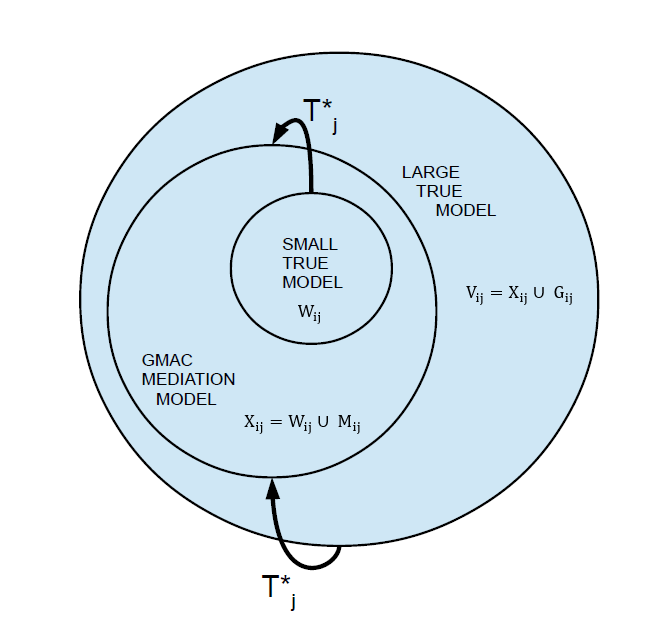
\includegraphics{C:/Users/Bruin/Documents/GitHub/MRPC_support/Manuscript/GMACwriteup_sim_diagram.png}
\caption{A visual depiction of the relationship between the simulation
models for the trans gene and the regression used for the mediation
test}
\end{figure}

\begin{figure}
\centering
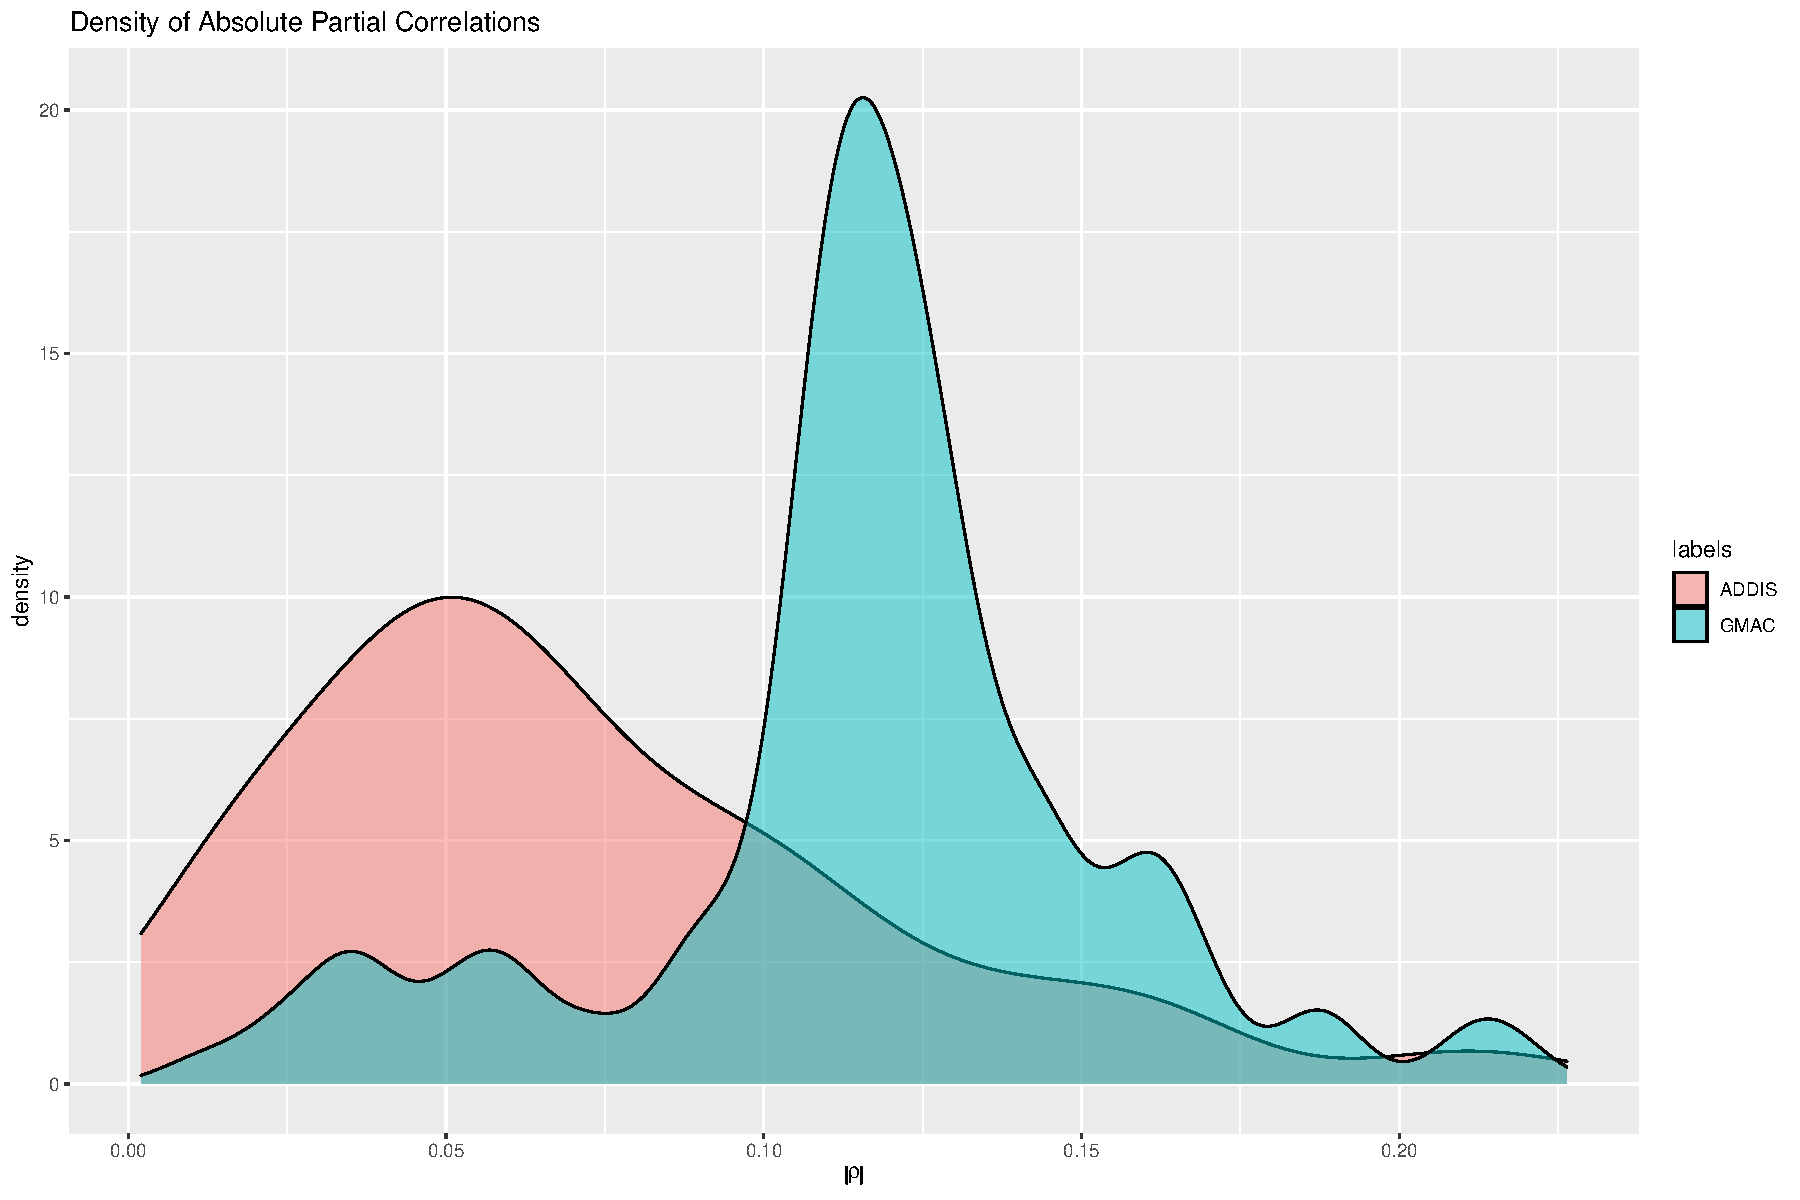
\includegraphics{GMACwriteup_files/figure-latex/unnamed-chunk-4-1.pdf}
\caption{A density plot for the absolute partial correlations to
demonstrate the strengthening of the adjusted relationship under the
GMAC mediation model.}
\end{figure}

\hypertarget{variance-across-tissues-plots}{%
\subsection{variance across tissues
plots}\label{variance-across-tissues-plots}}

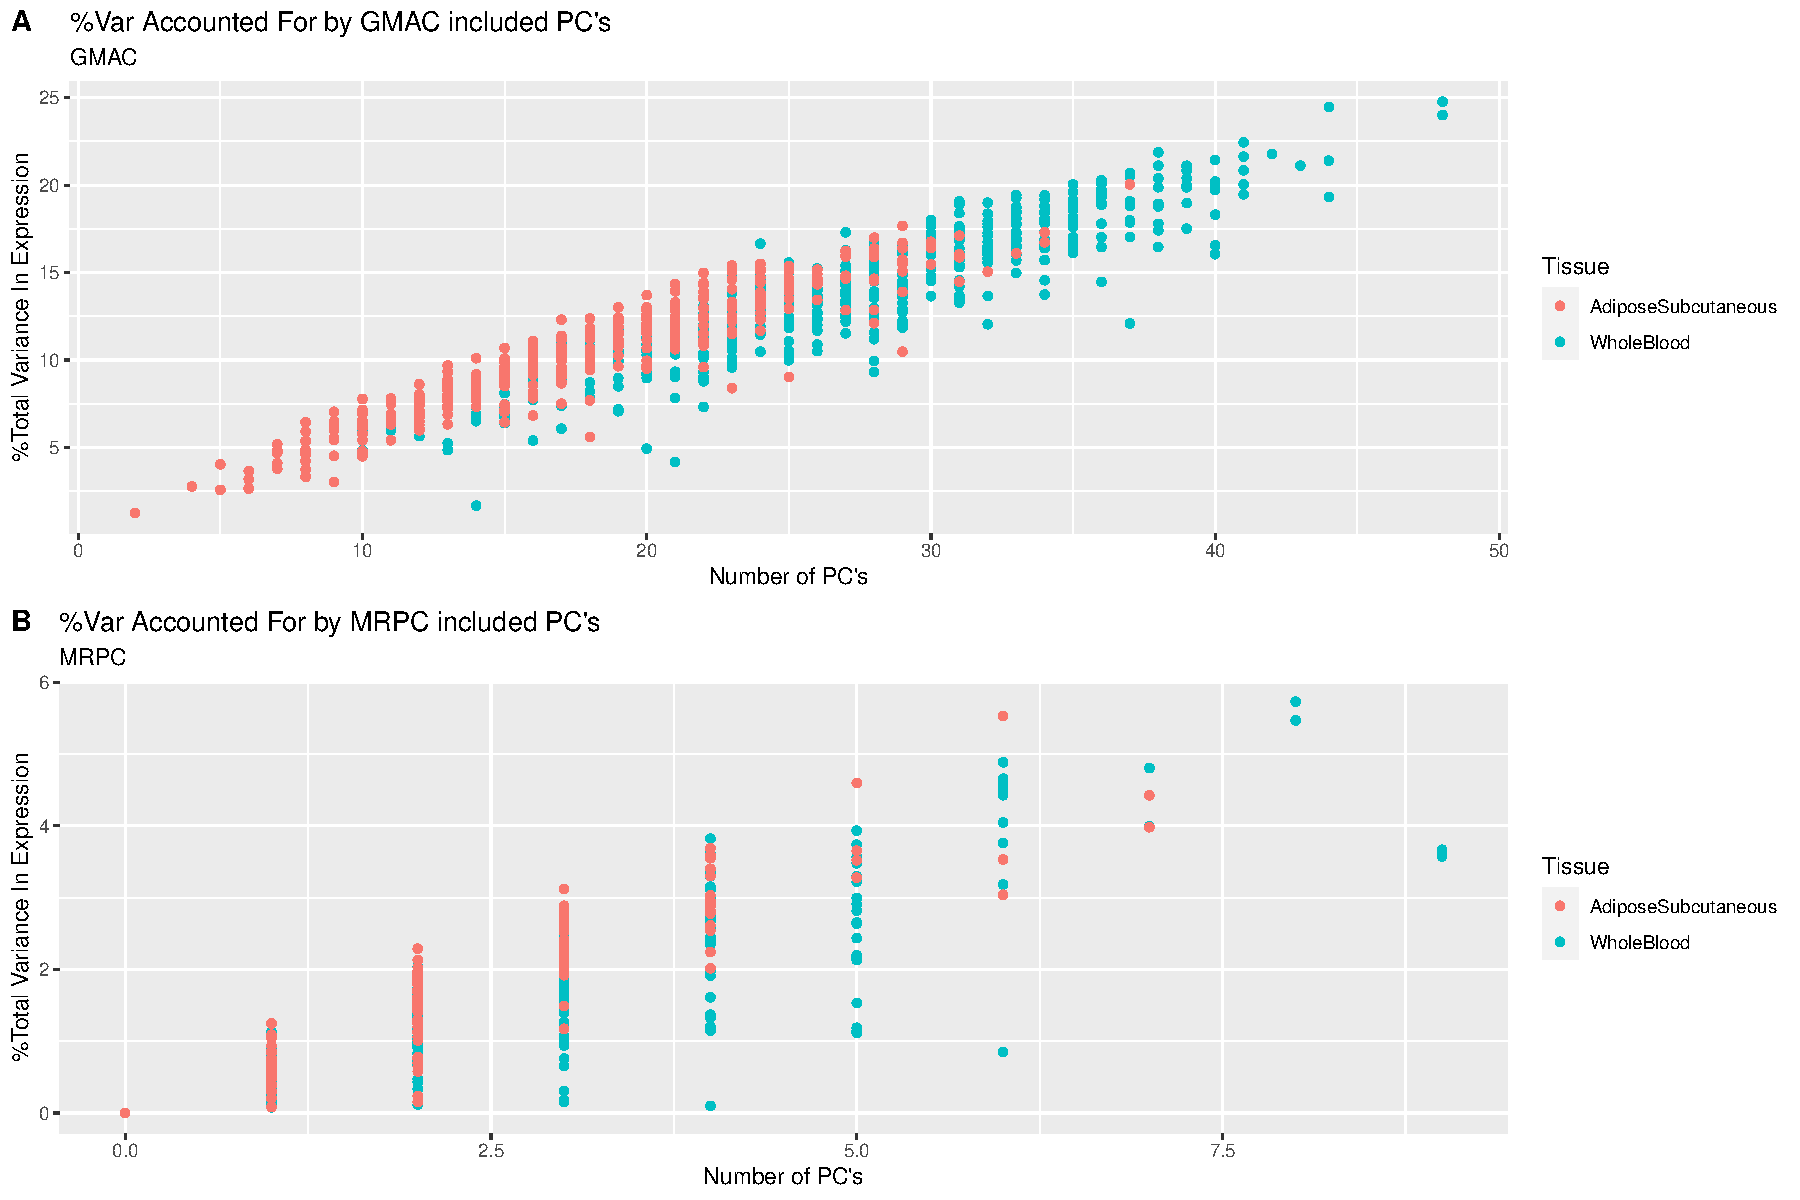
\includegraphics{GMACwriteup_files/figure-latex/unnamed-chunk-5-1.pdf}

\hypertarget{ltm-and-stm-plots}{%
\subsection{LTM and STM plots}\label{ltm-and-stm-plots}}

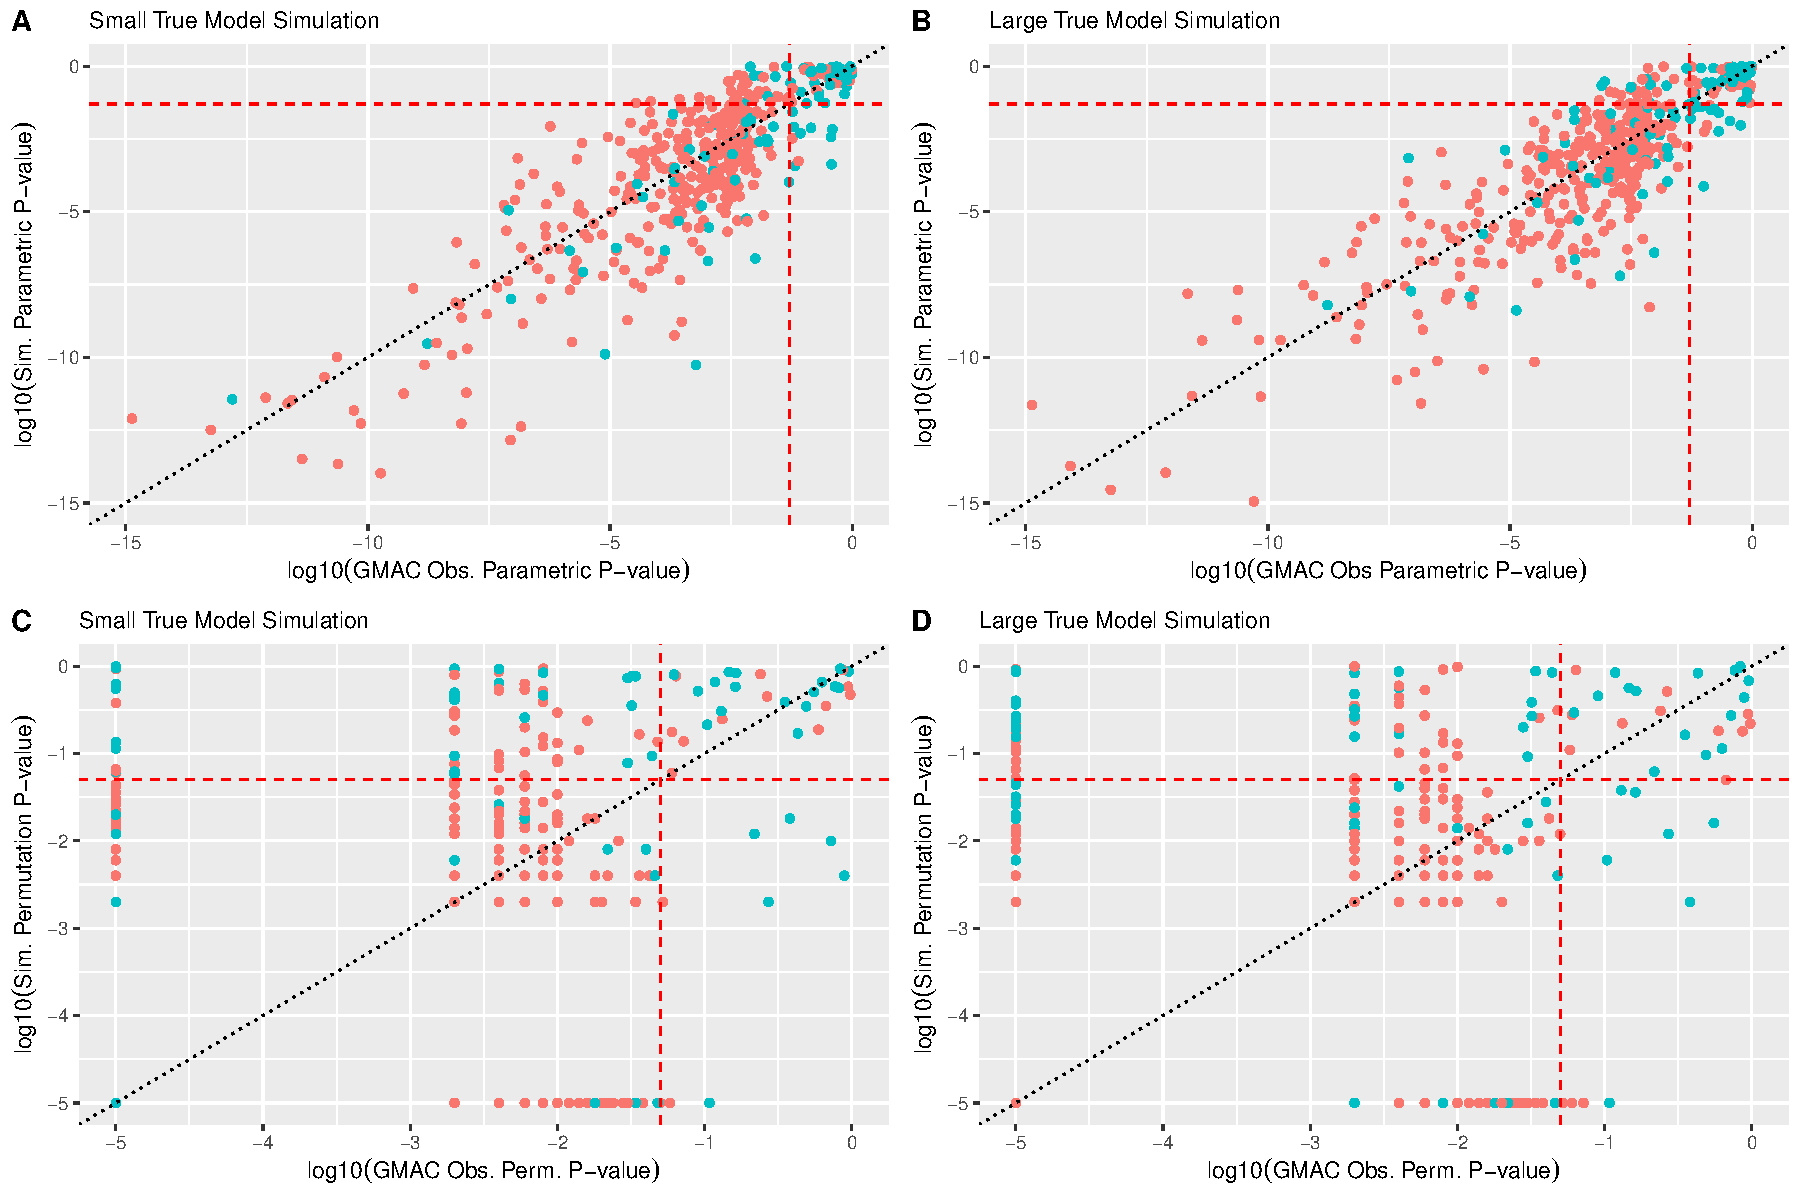
\includegraphics{GMACwriteup_files/figure-latex/unnamed-chunk-6-1.pdf}

\hypertarget{tgm-and-mrpc-plots}{%
\subsection{TGM and MRPC plots}\label{tgm-and-mrpc-plots}}

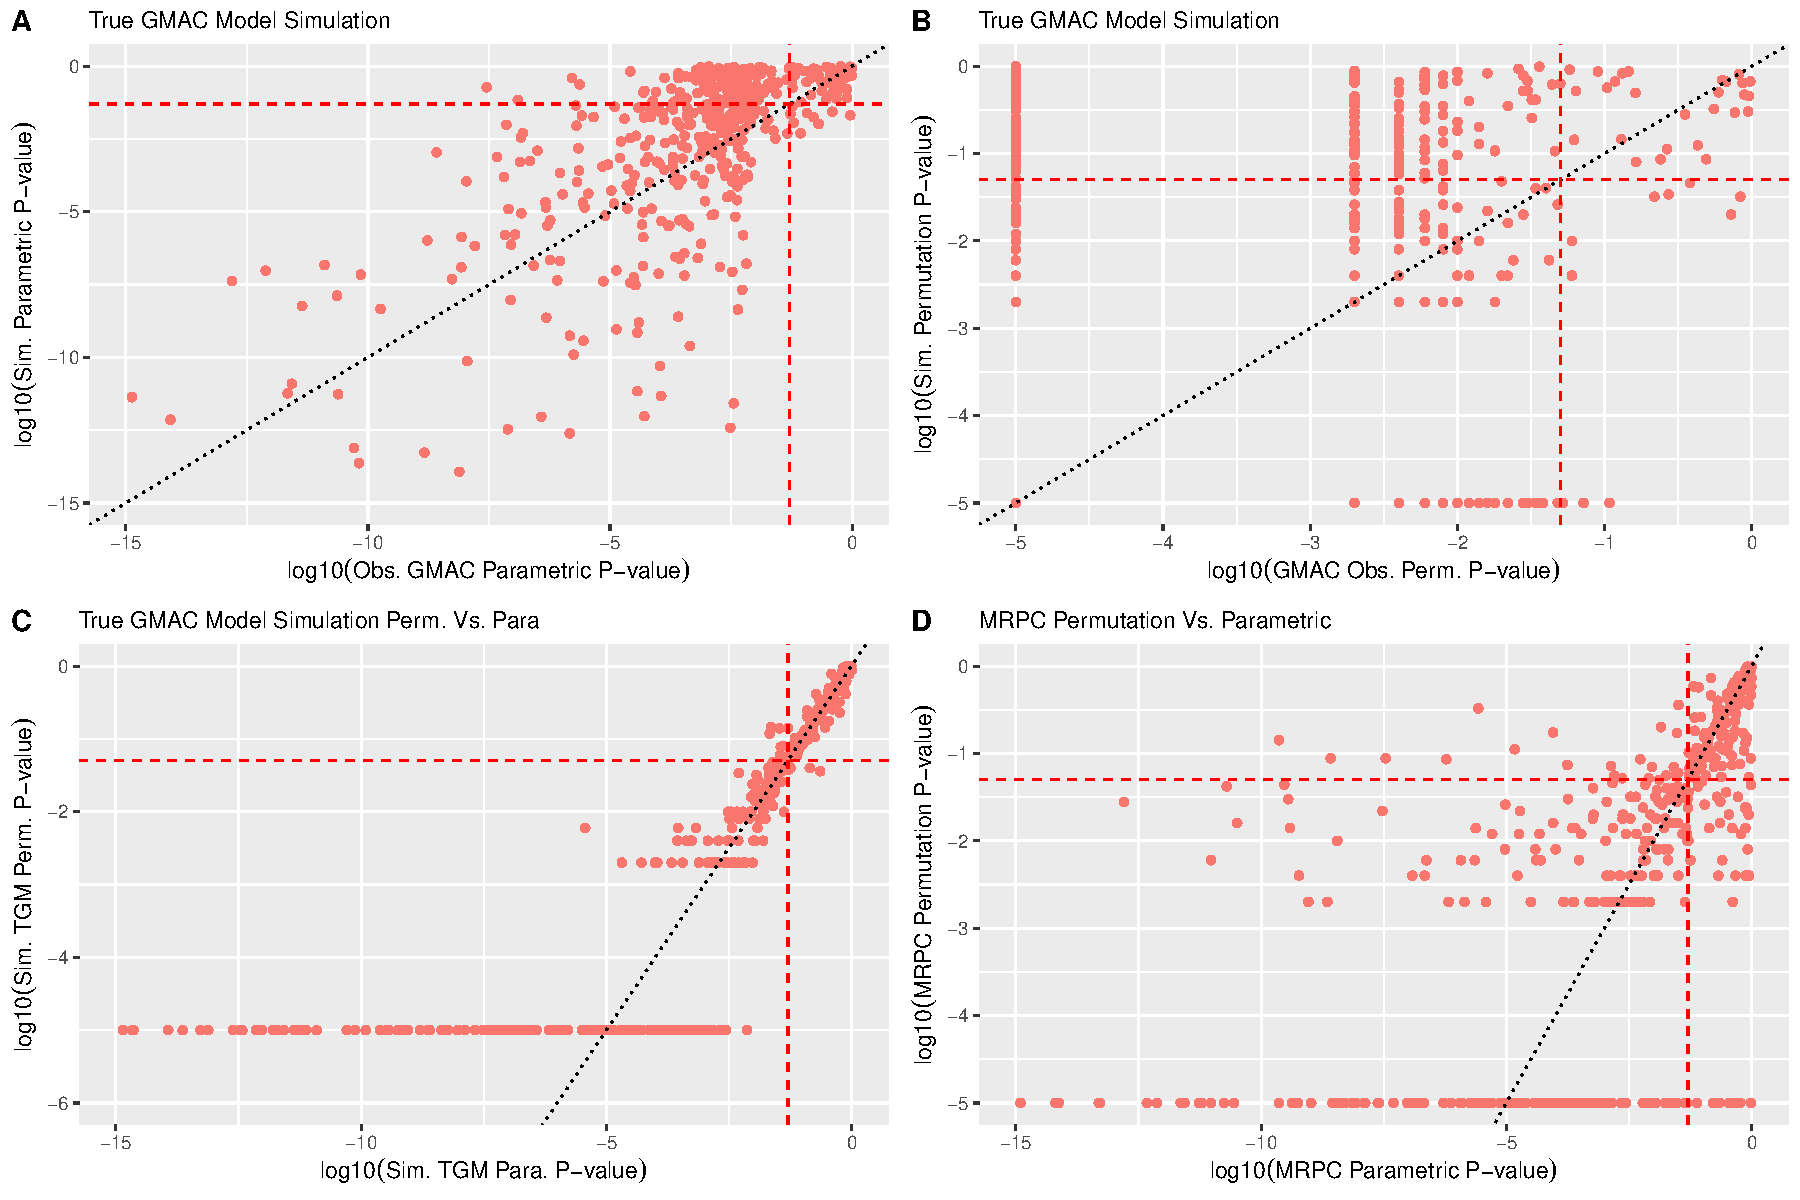
\includegraphics{GMACwriteup_files/figure-latex/unnamed-chunk-7-1.pdf}

\hypertarget{gss-and-gmac-plots}{%
\subsection{GSS and GMAC plots}\label{gss-and-gmac-plots}}

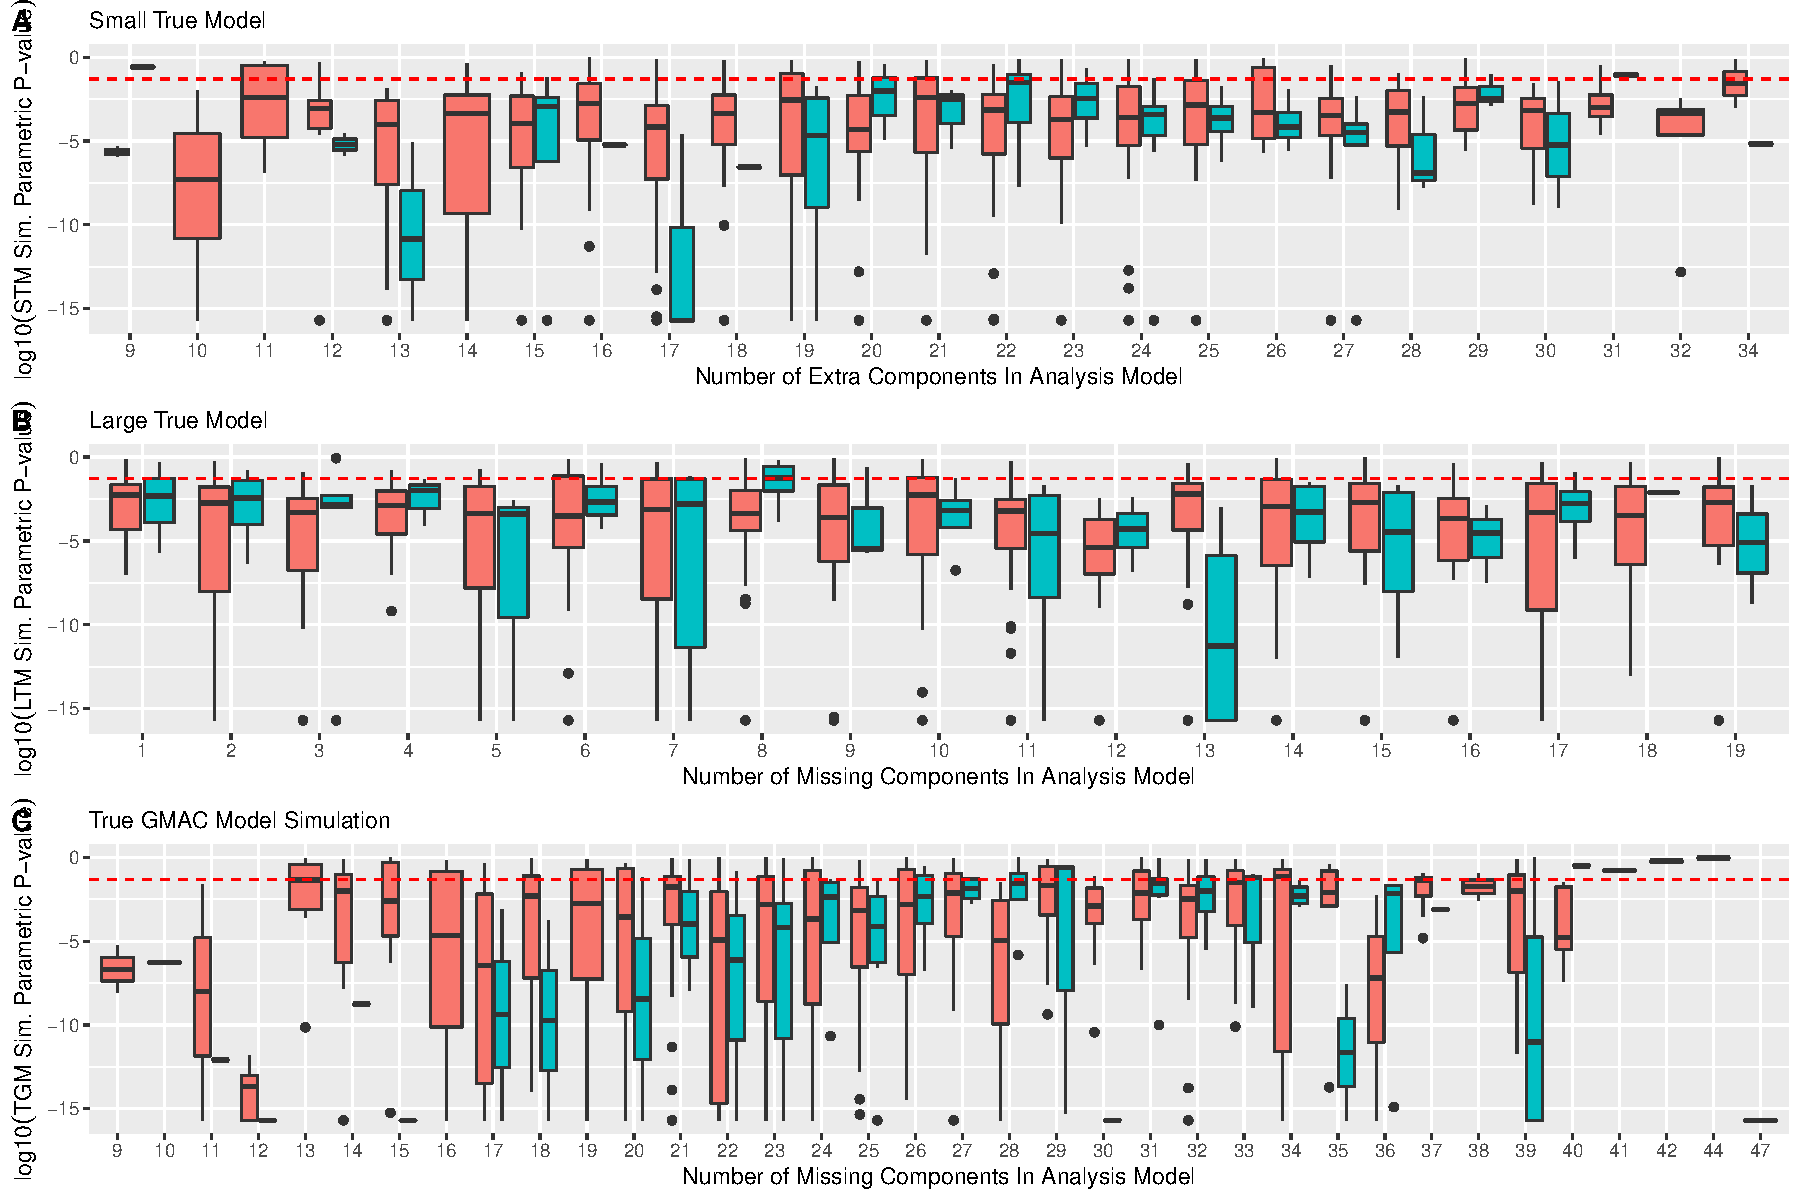
\includegraphics{GMACwriteup_files/figure-latex/unnamed-chunk-8-1.pdf}

\hypertarget{nominal-p-value-plots}{%
\subsection{Nominal P-value plots}\label{nominal-p-value-plots}}

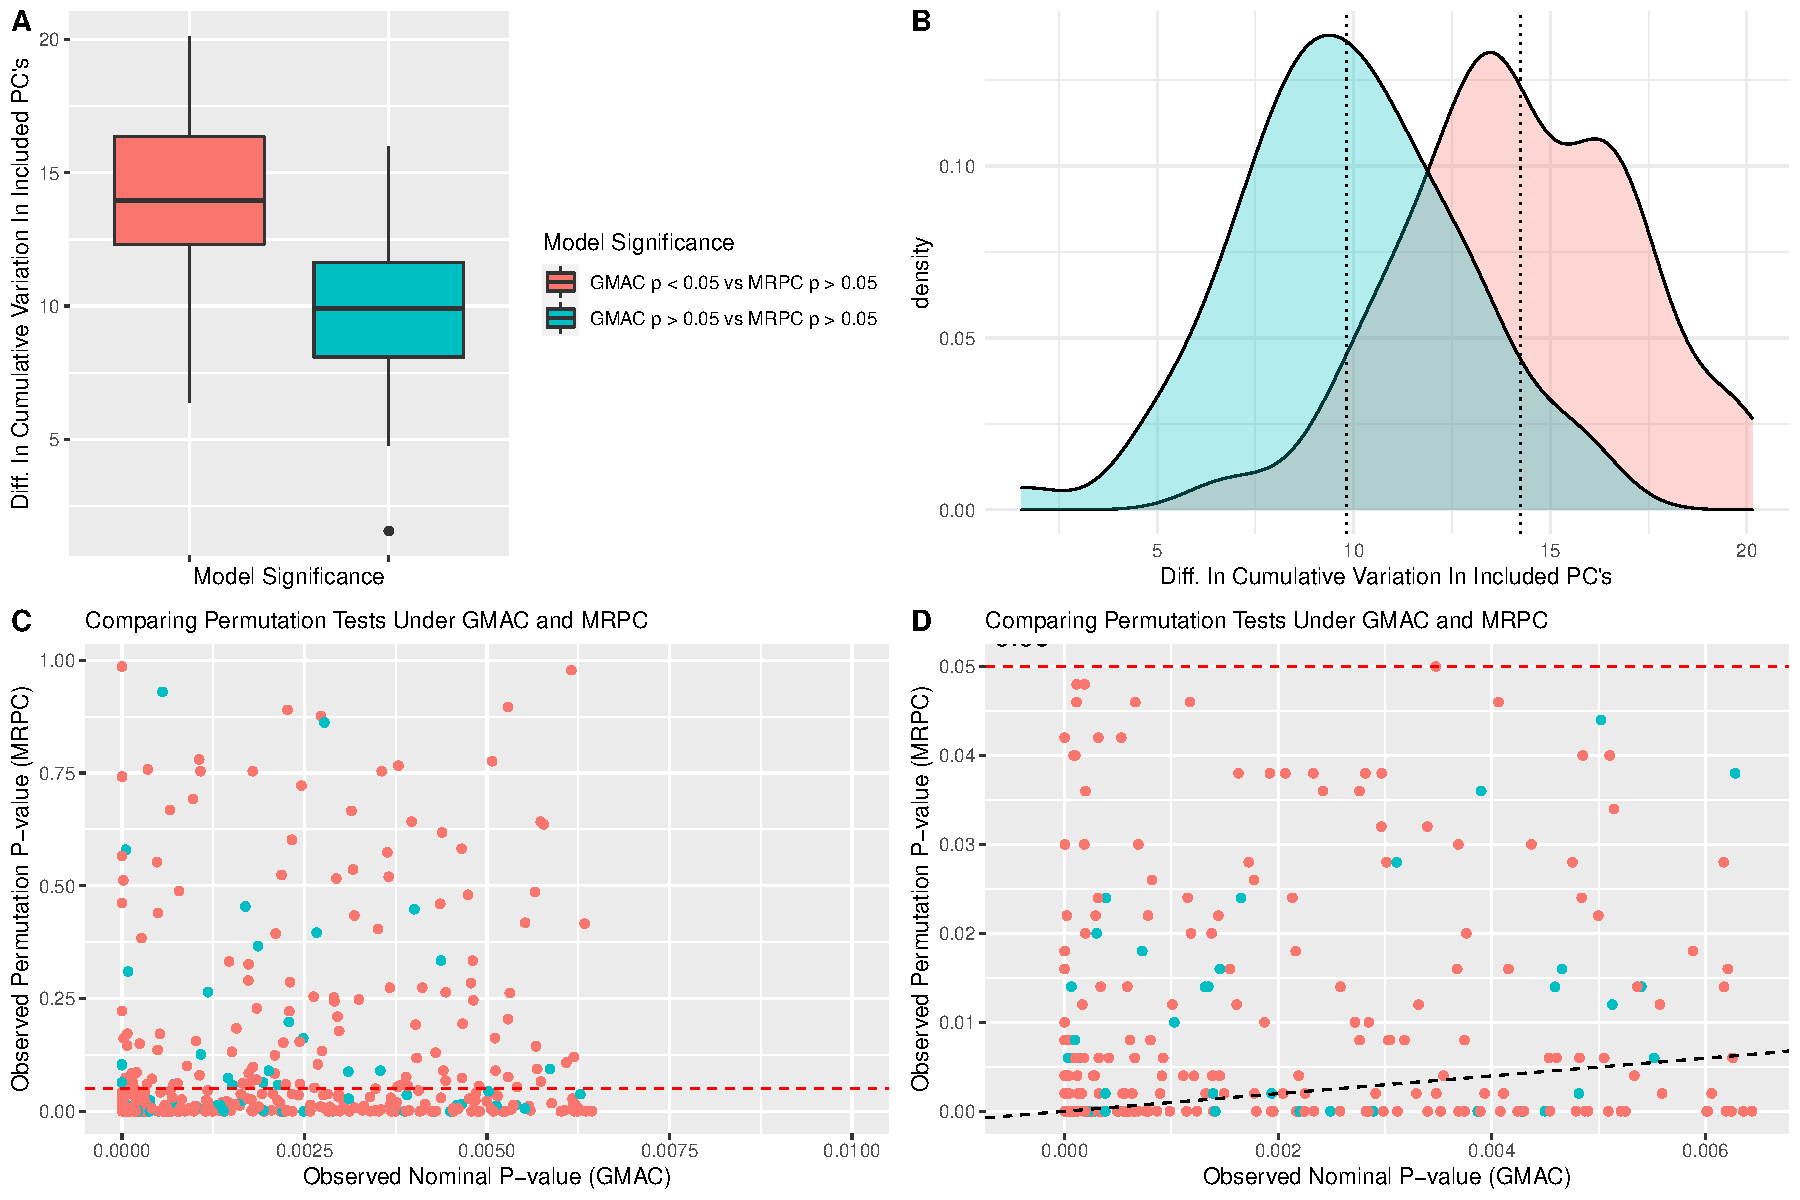
\includegraphics{GMACwriteup_files/figure-latex/unnamed-chunk-9-1.pdf}

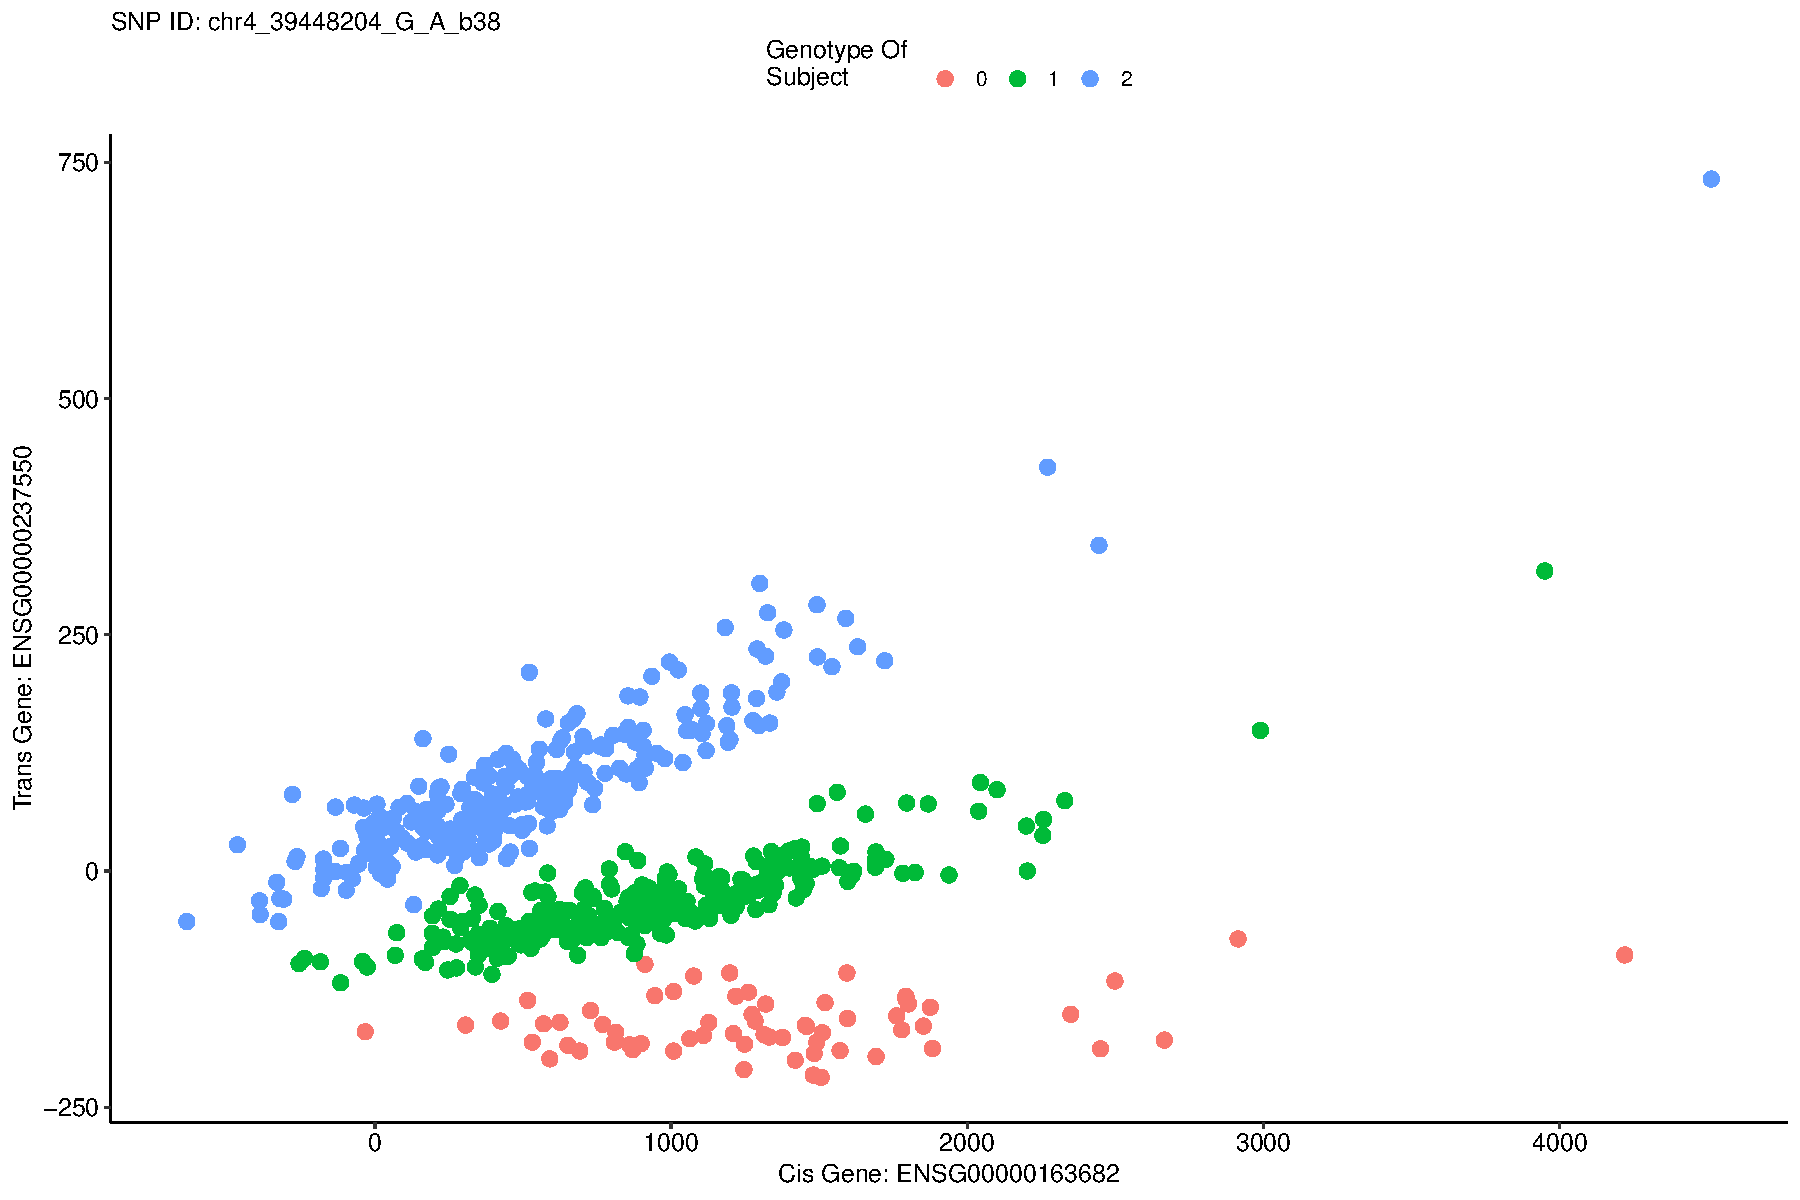
\includegraphics{GMACwriteup_files/figure-latex/unnamed-chunk-10-1.pdf}

\hypertarget{boxplots-for-pc-inclusion-differences}{%
\subsection{boxplots for PC inclusion
differences}\label{boxplots-for-pc-inclusion-differences}}

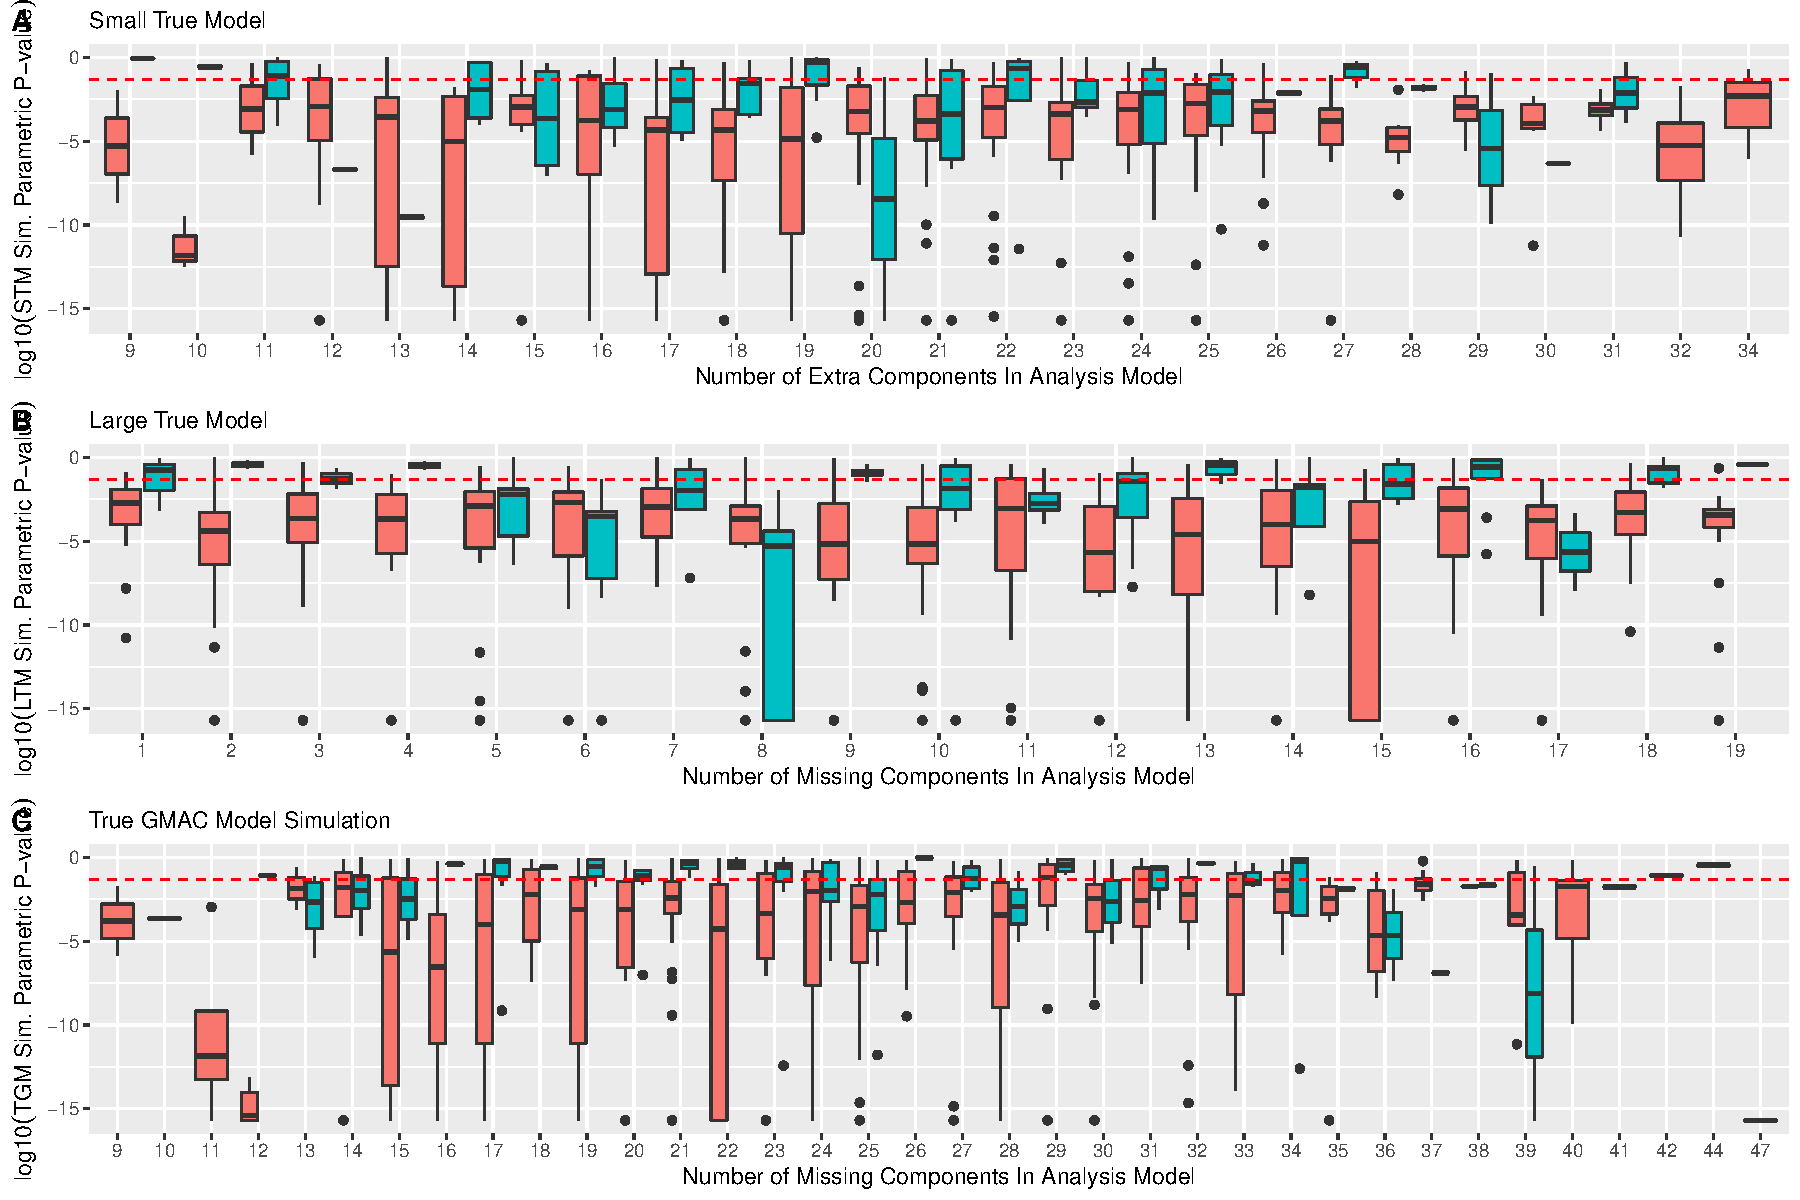
\includegraphics{GMACwriteup_files/figure-latex/unnamed-chunk-11-1.pdf}

\hypertarget{variation-differences-between-sig-and-non-sig-trios-gmacmrpc}{%
\subsection{variation differences between sig and non-sig trios
GMAC/MRPC}\label{variation-differences-between-sig-and-non-sig-trios-gmacmrpc}}

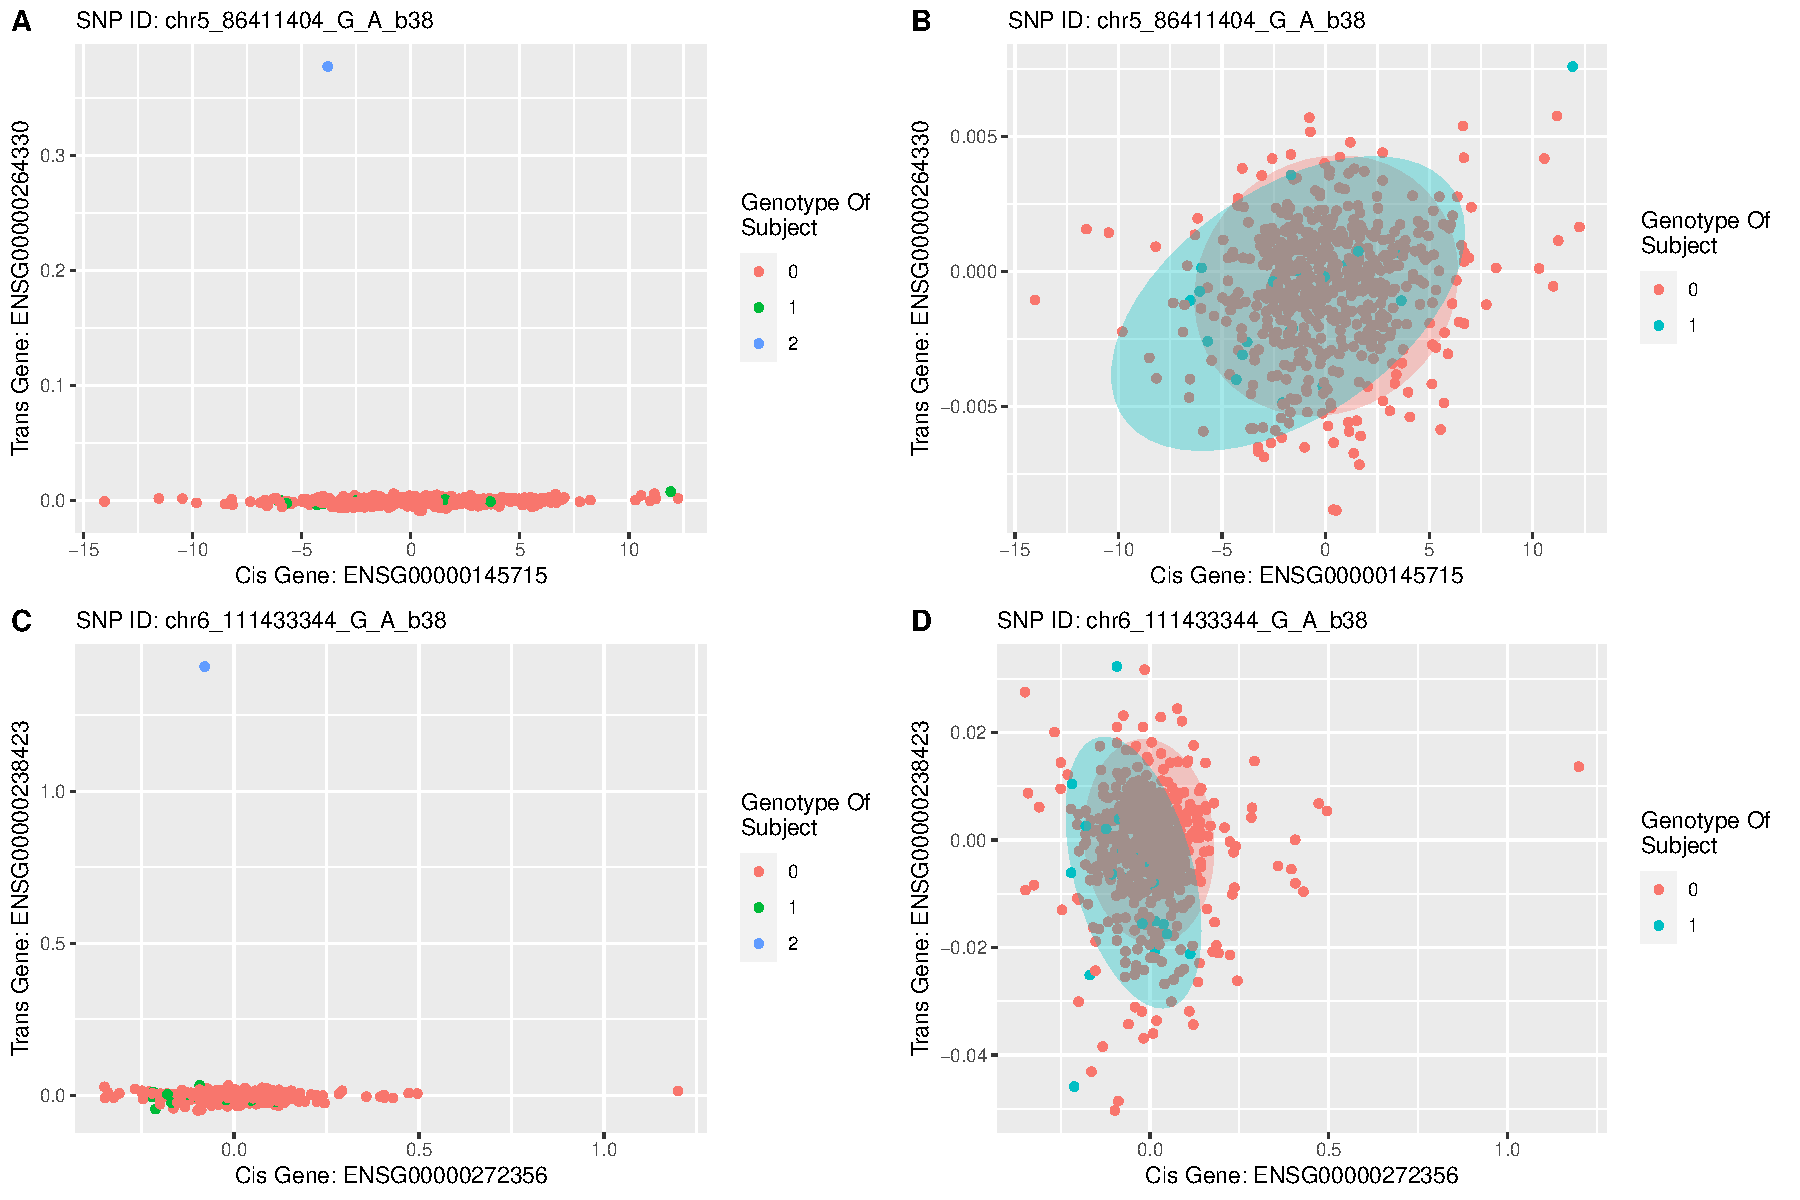
\includegraphics{GMACwriteup_files/figure-latex/unnamed-chunk-12-1.pdf}

\(\bullet\) Rare allele plots

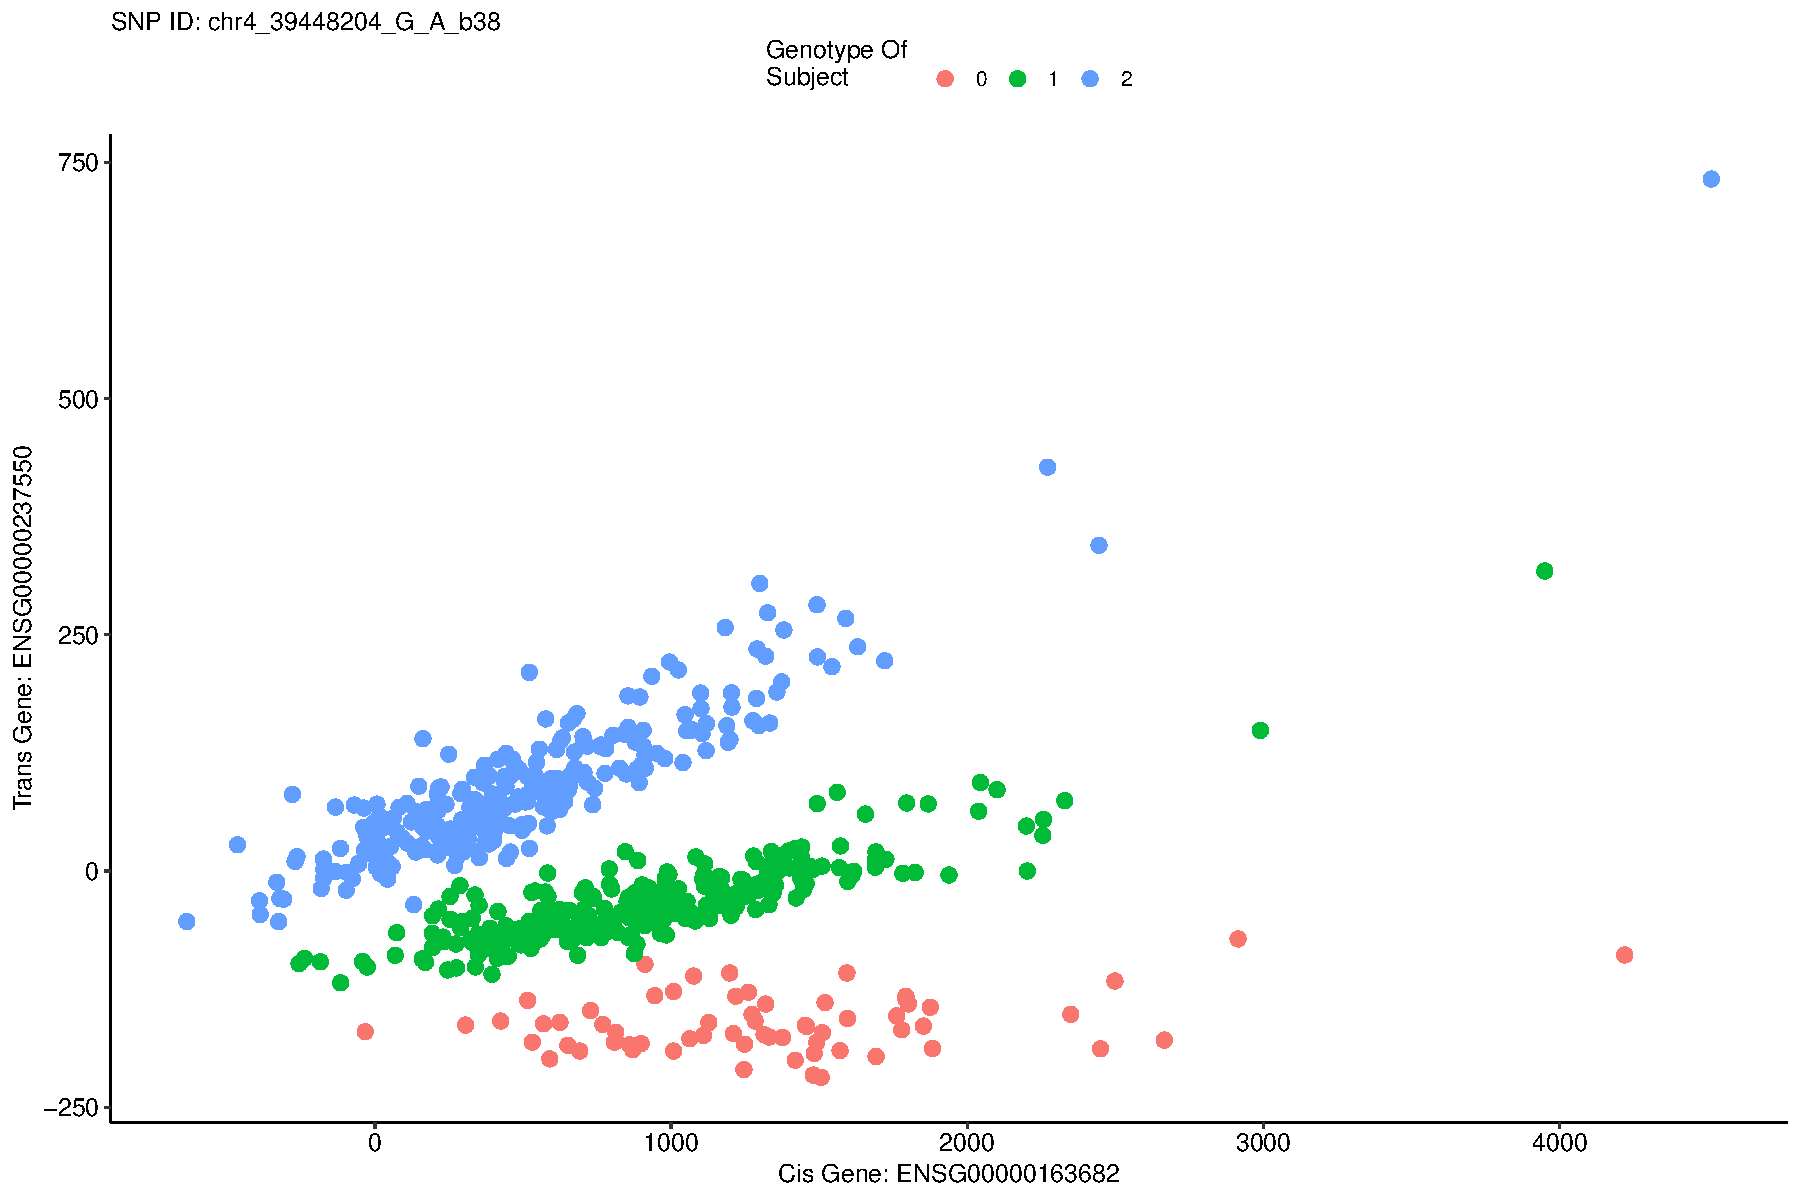
\includegraphics{GMACwriteup_files/figure-latex/unnamed-chunk-13-1.pdf}

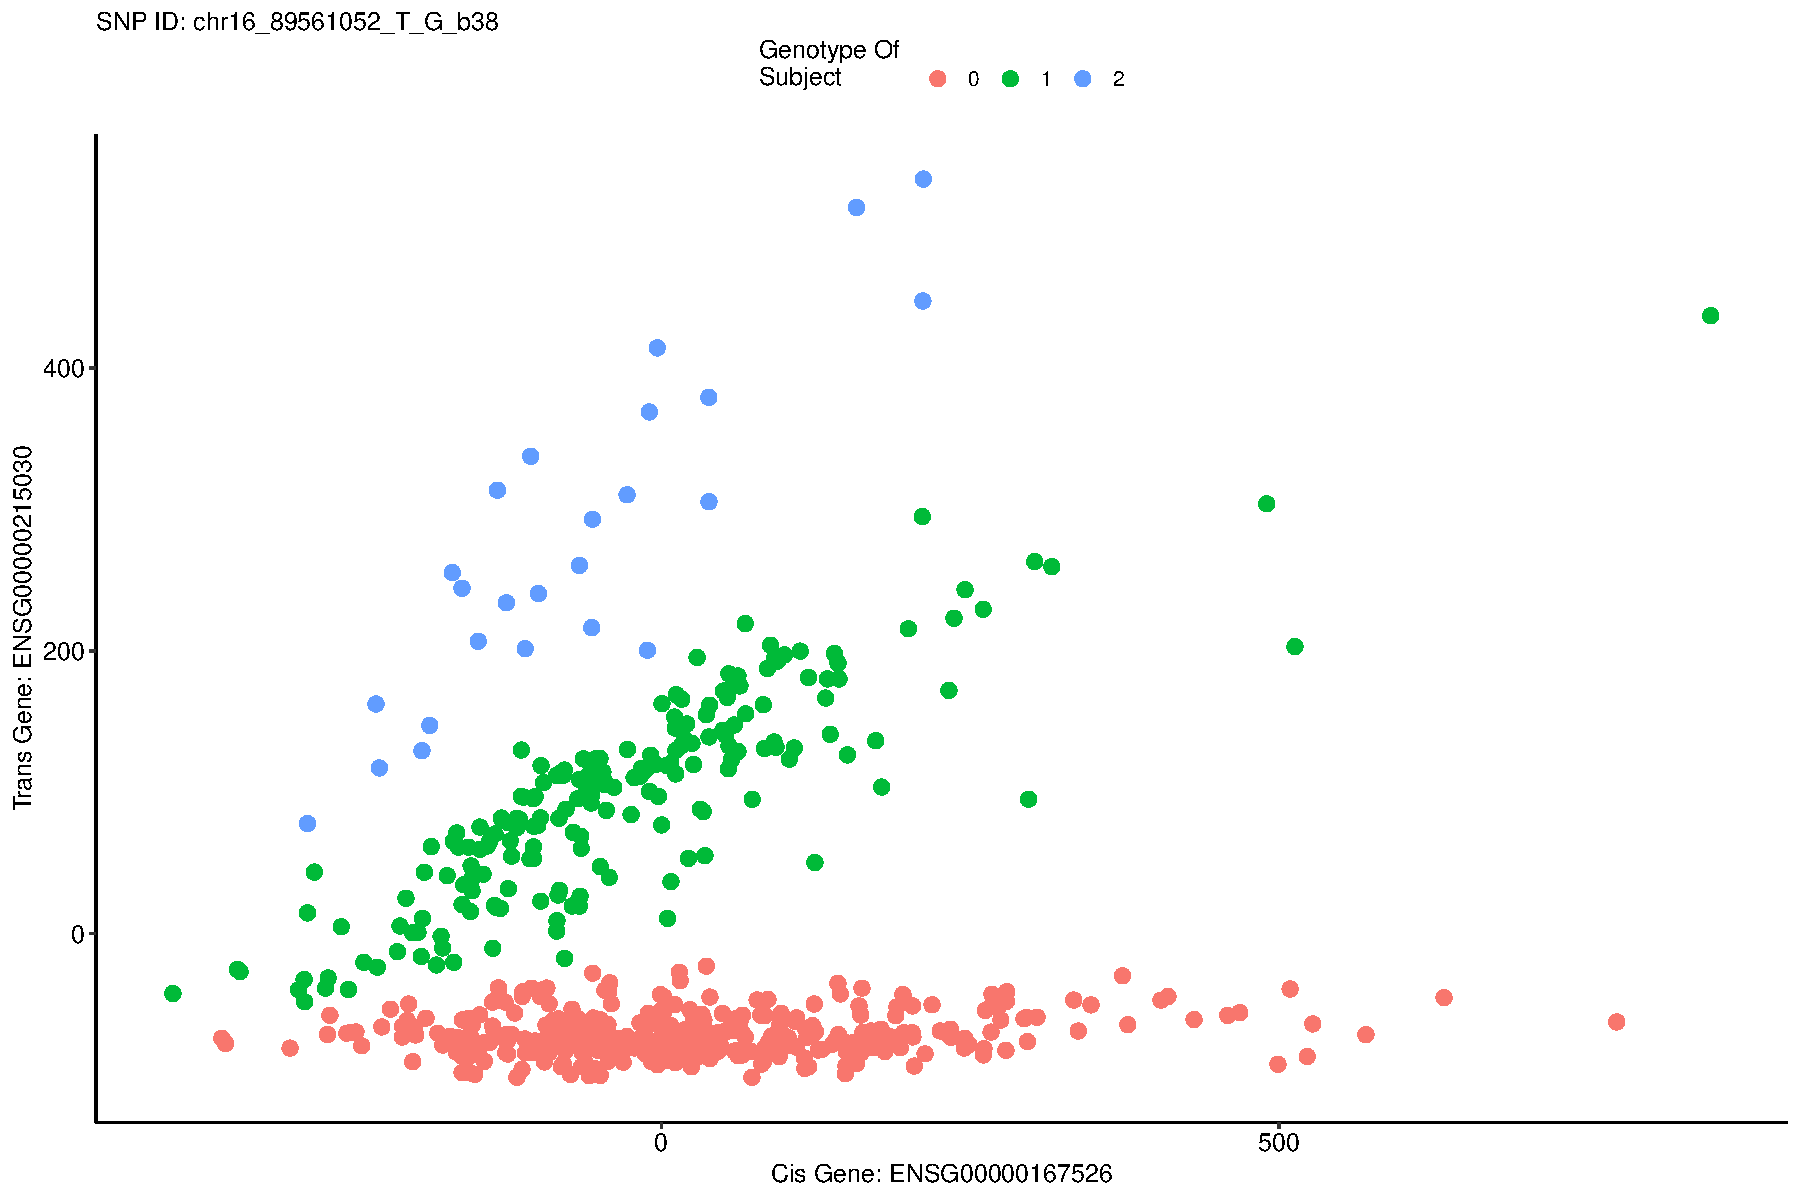
\includegraphics{GMACwriteup_files/figure-latex/unnamed-chunk-14-1.pdf}

\begin{figure}
\centering
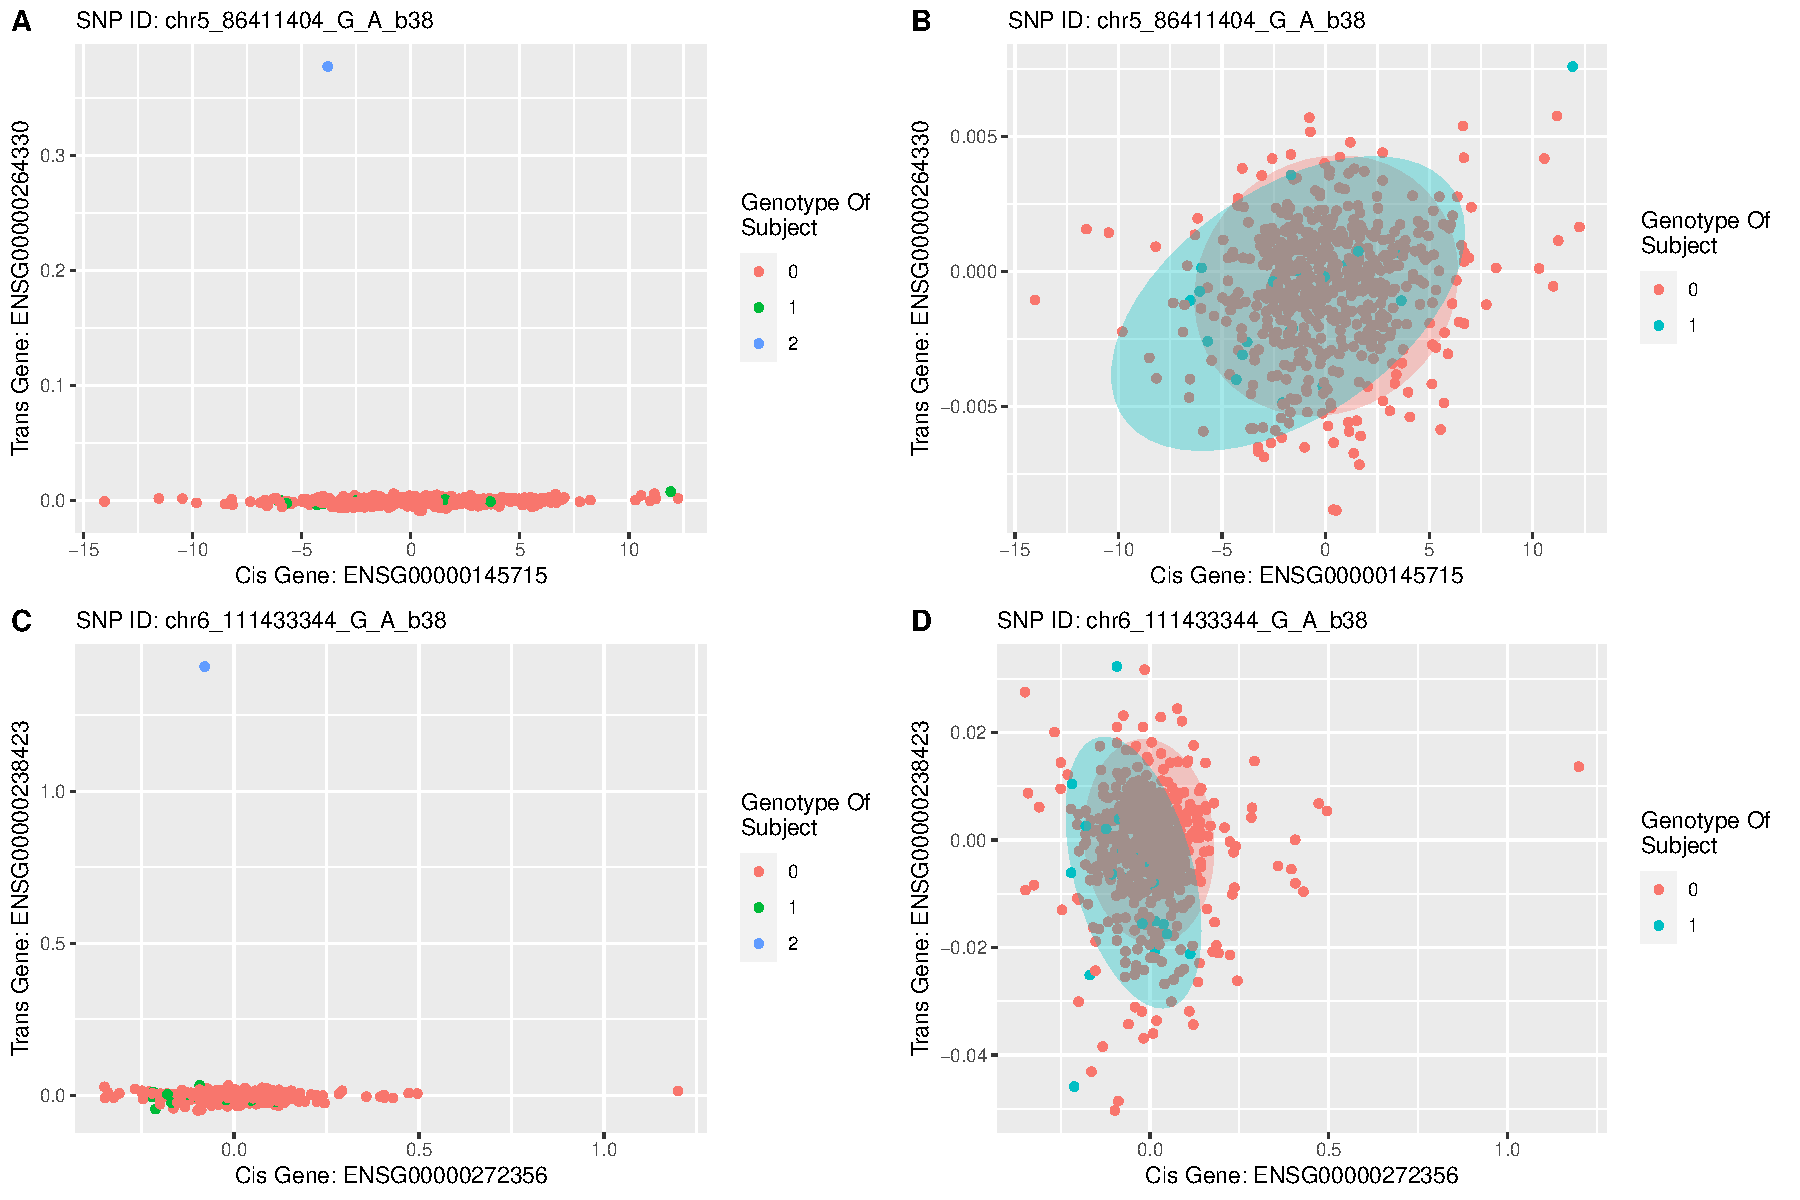
\includegraphics{GMACwriteup_files/figure-latex/unnamed-chunk-15-1.pdf}
\caption{\textbf{A} and \textbf{C}: Example scatter plots of trios from
subcutaneous adipose tissue and whole blood (respectively) with a rare
allele present in the sample: Note that 0 indicates individuals
homozygous for the reference allele, 1 indicates hetezygous individuals
and 2 indicates individuals who are homozygous for the alternative
(rare) allele. The apparent outlier represents a single individual in
the sample who was homozygous for the rare allele, and \textbf{B} and
\textbf{C} are the scatter plots with the point(s) for the
homozygous-alternative individuals removed and a confidence ellipse
calculated over the remaining homozygous-reference and heterzygous
individals.}
\end{figure}

\newpage
\section*{References}

\hypertarget{refs}{}
\leavevmode\hypertarget{ref-josse2016missmda}{}%
Josse, Julie, François Husson, and others. 2016. ``MissMDA: A Package
for Handling Missing Values in Multivariate Data Analysis.''
\emph{Journal of Statistical Software} 70 (1): 1--31.

\leavevmode\hypertarget{ref-yang2017identifying}{}%
Yang, Fan, Jiebiao Wang, Brandon L Pierce, Lin S Chen, François Aguet,
Kristin G Ardlie, Beryl B Cummings, et al. 2017. ``Identifying
Cis-Mediators for Trans-eQTLs Across Many Human Tissues Using Genomic
Mediation Analysis.'' \emph{Genome Research} 27 (11): 1859--71.

\end{document}
